% ============================================================================
% VigileEye — PFE Report
% Intelligent Video Surveillance System
% Humanized & Rewritten Version — Mohamed Yassin Ben Chayada & Omar Soussi
% ============================================================================
\documentclass[12pt,a4paper,oneside]{report}

% ─── Encoding & Fonts ────────────────────────────────────────────────────
\usepackage{fontspec}
\IfFontExistsTF{TeX Gyre Termes}{%
  \setmainfont{TeX Gyre Termes}%
}{%
  \setmainfont{Times New Roman}%
}

% ─── Language ────────────────────────────────────────────────────────────
\usepackage[english]{babel}

% ─── Page Geometry ───────────────────────────────────────────────────────
\usepackage[top=2cm,bottom=2cm,left=2.5cm,right=2cm,
            bindingoffset=0.5cm,headheight=14pt]{geometry}

% ─── Line Spacing ────────────────────────────────────────────────────────
\usepackage{setspace}
\onehalfspacing

% ─── Paragraph Style ─────────────────────────────────────────────────────
\usepackage{parskip}
\setlength{\parskip}{6pt}
\setlength{\parindent}{0.8cm}
\emergencystretch=1.5em

% ─── Graphics & Floats ───────────────────────────────────────────────────
\usepackage{graphicx}
\usepackage{float}
\usepackage{caption}
\captionsetup[figure]{position=below,font=small,labelfont=bf}
\captionsetup[table]{position=below,font=small,labelfont=bf}

% ─── Tables ──────────────────────────────────────────────────────────────
\usepackage{array}
\usepackage{booktabs}
\usepackage{longtable}
\usepackage{tabularx}
\usepackage{multirow}
\usepackage{makecell}
\usepackage{colortbl}

% ─── Charts & Diagrams ───────────────────────────────────────────────────
\usepackage{tikz}
\usepackage{pgfplots}
\pgfplotsset{compat=1.18}
\usetikzlibrary{patterns}

% ─── Lists ───────────────────────────────────────────────────────────────
\usepackage{enumitem}
\setlist[itemize]{label=\textbullet,nosep,leftmargin=1.5em}

% ─── Hyperlinks ───────────────────────────────────────────────────────────
\usepackage[colorlinks=true,
            linkcolor=black,
            citecolor=black,
            urlcolor=black,
            pdfborder={0 0 0}]{hyperref}

% ─── Headers & Footers ───────────────────────────────────────────────────
\usepackage{fancyhdr}
\pagestyle{fancy}
\fancyhf{}
\renewcommand{\headrulewidth}{0.4pt}
\renewcommand{\footrulewidth}{0.4pt}
\fancyhead[L]{\small\leftmark}
\fancyfoot[L]{\small VigileEye -- Intelligent Video Surveillance System}
\fancyfoot[R]{\small\thepage}
\fancypagestyle{plain}{%
  \fancyhf{}
  \renewcommand{\headrulewidth}{0pt}
  \renewcommand{\footrulewidth}{0.4pt}
  \fancyfoot[L]{\small VigileEye -- Intelligent Video Surveillance System}
  \fancyfoot[R]{\small\thepage}
}

% ─── Chapter / Section Formatting ────────────────────────────────────────
\usepackage{titlesec}
\renewcommand{\thechapter}{\Roman{chapter}}

\titleformat{\chapter}[display]
  {\normalfont\fontsize{16}{19}\bfseries}
  {Chapter \thechapter}{12pt}{\fontsize{16}{19}\bfseries}
\titlespacing*{\chapter}{0pt}{-20pt}{20pt}

\titleformat{\section}
  {\normalfont\fontsize{14}{17}\bfseries}{\thesection}{1em}{}
\titlespacing*{\section}{0pt}{12pt}{6pt}

\titleformat{\subsection}
  {\normalfont\fontsize{12}{15}\bfseries}{\thesubsection}{1em}{}
\titlespacing*{\subsection}{0pt}{10pt}{4pt}

\titleformat{\subsubsection}
  {\normalfont\fontsize{12}{14}\bfseries\itshape}{\thesubsubsection}{1em}{}
\titlespacing*{\subsubsection}{0pt}{8pt}{3pt}

\usepackage{needspace}

% ─── Miscellaneous ───────────────────────────────────────────────────────
\usepackage{url}
\usepackage{xcolor}
\usepackage{microtype}
\usepackage{amssymb}
\setcounter{tocdepth}{3}
\setcounter{secnumdepth}{3}

% ─── Prevent orphan titles ────────────────────────────────────────────────
\usepackage{etoolbox}
\preto\section{\needspace{4\baselineskip}}
\preto\subsection{\needspace{3\baselineskip}}
\preto\subsubsection{\needspace{3\baselineskip}}

% ─────────────────────────────────────────────────────────────────────────
\begin{document}

% ══════════════════════════════════════════════════════════════════════════
%  COVER PAGE
% ══════════════════════════════════════════════════════════════════════════
\begin{titlepage}
\begin{center}
\textbf{General Directorate of Technological Studies}\\[4pt]
\textbf{Higher Institute of Technological Studies of Mahdia}\\[6pt]
\rule{\textwidth}{0.4pt}\\[12pt]
{\small ISET Mahdia, Avenue Elmourouj 5111 Hiboun Mahdia Tunisie\\
T\'{e}l\,: (+216)73 68 34 07 -- (+216)73 68 34 10 \quad Fax\,: (+216)73 68 33 99}\\[24pt]
{\Large\bfseries FINAL YEAR PROJECT}\\[12pt]
{\normalsize PRESENTED TO OBTAIN THE TITLE:}\\[6pt]
{\large\bfseries NATIONAL LICENSE DEGREE}\\[6pt]
{\normalsize In Information Technology}\\[4pt]
{\normalsize Course: Development of Information Systems (DSI)}\\[20pt]
{\normalsize Realized by: \textbf{Mohamed Yassin Ben Chayada and Omar Soussi}}\\[24pt]
{\normalsize DEFENDED ON [DATE] BEFORE THE EXAMINATION COMMITTEE:}\\[10pt]
\begin{tabular}{ll}
Mrs/Mr: [President Name]    & President \\
Mrs/Mr: [Examiner Name]     & Examiner  \\
Dr: Mohamed Aymen Charrada  & ISET Supervisor \\
Mr: Mahdi Matar             & Company Supervisor \\
\end{tabular}\\[20pt]
{\normalsize A.Y.~: 2024--2025}\\[24pt]
\rule{\textwidth}{0.8pt}\\[10pt]
{\LARGE\bfseries Project Topic}\\[8pt]
{\Large\bfseries VigileEye -- Intelligent Video Surveillance System}\\[8pt]
\rule{\textwidth}{0.8pt}\\[10pt]
{\normalsize Project Code~: DSI[XX]}
\end{center}
\end{titlepage}

% ══════════════════════════════════════════════════════════════════════════
%  PRELIMINARY PAGES
% ══════════════════════════════════════════════════════════════════════════
\pagenumbering{gobble}

\newpage\thispagestyle{empty}
\begin{center}\vspace*{5cm}
{\Large\bfseries Internship Certificate}\\[2cm]
{\normalsize [Insert internship certificate here]}
\end{center}

\newpage\thispagestyle{empty}
\begin{center}\vspace*{5cm}
{\Large\bfseries Activity Sheets}\\[2cm]
{\normalsize [Insert activity sheets here]}
\end{center}

\newpage\thispagestyle{empty}
\begin{center}\vspace*{5cm}
{\Large\bfseries Evaluation Sheet}\\[2cm]
{\normalsize [Insert evaluation sheet here]}
\end{center}

% ─── Dedication — Omar Soussi ─────────────────────────────────────────────
\newpage\thispagestyle{empty}
\begin{center}
\vspace*{2cm}
{\Large\bfseries Dedication}\\[0.3cm]
{\normalsize\itshape Omar Soussi}\\[1.5cm]
\end{center}
{\itshape
\hspace{0.8cm}To my mother and father — honestly, I don't think I have the words to fully express what you've given me. You carried me through every difficult stretch of this journey, sometimes more than you even knew. Your patience, your belief in me even when I doubted myself, the way you'd ask how things were going at IBSOFT every single evening — that stuff kept me going more than anything. Everything I achieve has your names written somewhere inside it.

\hspace{0.8cm}To my brothers, cousins, and friends who were always around, whether to celebrate a small win or just sit with me through a rough patch — thank you for making this period feel less lonely and a lot more meaningful.

\hspace{0.8cm}To the professors at ISET Mahdia who shaped how I think about technology and about work: Dr Mohamed Aymen Charrada, who never made us feel like we were bothering him no matter how many questions we had; Ms.\ Lobna Ben Rhouma, Ms.\ Nahla Sassi, Mr.\ Wahid Bannour, and Mr.\ Hafedh Boukthir — your teaching left a mark I'll carry a long time.

\hspace{0.8cm}This work is for all of you.
}

% ─── Dedication — Mohamed Yassin Ben Chayada ─────────────────────────────
\newpage\thispagestyle{empty}
\begin{center}
\vspace*{2cm}
{\Large\bfseries Dedication}\\[0.3cm]
{\normalsize\itshape Mohamed Yassin Ben Chayada}\\[1.5cm]
\end{center}
{\itshape
\hspace{0.8cm}To my parents — you are the reason I made it to this page. Every late night I spent debugging something that made no sense, every moment I wanted to give up and just take the easy route, I remembered that you never once took the easy route for me. Your love is not something I can repay, only try to reflect in everything I do.

\hspace{0.8cm}To my family and friends who showed up consistently throughout these four months — whether with a phone call, a message, or just being present — you all mattered more than you probably realize.

\hspace{0.8cm}To Ms.\ B.\ Lobna, whose mentorship went far beyond what any class schedule could contain: you pushed us to aim higher and believe in our own ideas. That kind of support is rare and I genuinely appreciate it.

\hspace{0.8cm}To Dr Mohamed Aymen Charrada, Mr.\ Mahdi Matar, and the whole team at IBSOFT who took us in and treated us like real engineers from day one — thank you for the environment, the feedback, and the trust.

\hspace{0.8cm}This work is dedicated to all of you, with real gratitude.
}

% ─── Acknowledgments ─────────────────────────────────────────────────────
\newpage\thispagestyle{empty}
\begin{center}\vspace*{1.5cm}
{\Large\bfseries Acknowledgments}\\[1cm]
\end{center}

\hspace{0.8cm}First and above all, we thank Allah for giving us the strength, the clarity of mind, and the perseverance to push this project all the way through to completion. There were moments where things felt genuinely stuck, and looking back, we're grateful for every one of those obstacles because they made the final result mean something.

\hspace{0.8cm}We want to express our deepest thanks to Dr Mohamed Aymen Charrada, our academic supervisor, who guided us throughout this work with a patience and availability that we deeply appreciated. He never made us feel rushed or dismissed, and his feedback always pushed us in the right direction — even when it meant going back and rethinking something we thought was finished.

\hspace{0.8cm}A warm thank you also goes to Mr.\ Mahdi Matar, founder of IBSOFT, for welcoming us into his company and giving us a real professional environment to grow in. The way he trusted us with actual responsibilities from the very beginning was something we didn't take lightly. His practical perspective helped us understand the gap between how things are taught and how they actually get built, and that shift in thinking was invaluable.

\hspace{0.8cm}Finally, our thanks go to the members of the jury for taking the time to read and evaluate this work. We hope it reflects the care we put into it.

% ══════════════════════════════════════════════════════════════════════════
%  TABLE OF CONTENTS, LOF, LOT
% ══════════════════════════════════════════════════════════════════════════
\newpage\pagenumbering{roman}
\tableofcontents
\newpage\listoffigures
\newpage\listoftables

% ─── Abbreviations ───────────────────────────────────────────────────────
\newpage
\chapter*{Abbreviations}
\addcontentsline{toc}{chapter}{Abbreviations}
\markboth{Abbreviations}{}

\textbf{Architecture \& Design Patterns}\\[4pt]
\begin{tabular}{@{}p{3cm}l@{}}
\textbf{API}     & Application Programming Interface \\
\textbf{CRUD}    & Create, Read, Update, Delete \\
\textbf{DTO}     & Data Transfer Object \\
\textbf{MVVM}    & Model--View--ViewModel \\
\textbf{ORM}     & Object-Relational Mapping \\
\textbf{RBAC}    & Role-Based Access Control \\
\textbf{REST}    & Representational State Transfer \\
\textbf{SFU}     & Selective Forwarding Unit \\
\end{tabular}

\vspace{12pt}
\textbf{Security}\\[4pt]
\begin{tabular}{@{}p{3cm}l@{}}
\textbf{2FA}     & Two-Factor Authentication \\
\textbf{JWT}     & JSON Web Token \\
\textbf{OTP}     & One-Time Password \\
\textbf{OAuth}   & Open Authorization \\
\textbf{HTTPS}   & HyperText Transfer Protocol Secure \\
\end{tabular}

\vspace{12pt}
\textbf{Communication Protocols}\\[4pt]
\begin{tabular}{@{}p{3cm}l@{}}
\textbf{HLS}     & HTTP Live Streaming \\
\textbf{HTTP}    & HyperText Transfer Protocol \\
\textbf{RTMP}    & Real-Time Messaging Protocol \\
\textbf{RTSP}    & Real-Time Streaming Protocol \\
\textbf{RTP}     & Real-time Transport Protocol \\
\textbf{SDP}     & Session Description Protocol \\
\textbf{SMTP}    & Simple Mail Transfer Protocol \\
\textbf{WebRTC}  & Web Real-Time Communication \\
\textbf{WHEP}    & WebRTC-HTTP Egress Protocol \\
\textbf{WHIP}    & WebRTC-HTTP Ingress Protocol \\
\end{tabular}

\vspace{12pt}
\textbf{Technologies \& Frameworks}\\[4pt]
\begin{tabular}{@{}p{3cm}l@{}}
\textbf{AI}      & Artificial Intelligence \\
\textbf{CSS}     & Cascading Style Sheets \\
\textbf{GO}      & Go (Golang) -- statically typed compiled language \\
\textbf{HTML}    & HyperText Markup Language \\
\textbf{IoT}     & Internet of Things \\
\textbf{JSX}     & JavaScript XML \\
\textbf{ONVIF}   & Open Network Video Interface Forum \\
\textbf{YOLO}    & You Only Look Once (real-time object detection model) \\
\end{tabular}

\vspace{12pt}
\textbf{Database \& Storage}\\[4pt]
\begin{tabular}{@{}p{3cm}l@{}}
\textbf{DB}      & Database \\
\textbf{DVR}     & Digital Video Recorder \\
\textbf{NVR}     & Network Video Recorder \\
\textbf{SQL}     & Structured Query Language \\
\textbf{UUID}    & Universally Unique Identifier \\
\end{tabular}

\vspace{12pt}
\textbf{Streaming \& Multimedia}\\[4pt]
\begin{tabular}{@{}p{3cm}l@{}}
\textbf{FPS}     & Frames Per Second \\
\textbf{GPS}     & Global Positioning System \\
\textbf{ICE}     & Interactive Connectivity Establishment \\
\textbf{JPEG}    & Joint Photographic Experts Group \\
\textbf{MP4}     & MPEG-4 Part 14 (video container format) \\
\textbf{NAT}     & Network Address Translation \\
\textbf{STUN}    & Session Traversal Utilities for NAT \\
\textbf{TURN}    & Traversal Using Relays around NAT \\
\end{tabular}

\vspace{12pt}
\textbf{Project Management \& Tools}\\[4pt]
\begin{tabular}{@{}p{3cm}l@{}}
\textbf{CI/CD}   & Continuous Integration / Continuous Delivery \\
\textbf{IDE}     & Integrated Development Environment \\
\textbf{UML}     & Unified Modeling Language \\
\textbf{VMS}     & Video Management Software \\
\end{tabular}

% ══════════════════════════════════════════════════════════════════════════
%  MAIN CONTENT
% ══════════════════════════════════════════════════════════════════════════
\newpage\pagenumbering{arabic}\setcounter{page}{1}

% ══════════════════════════════════════════════════════════════════════════
%  GENERAL INTRODUCTION
% ══════════════════════════════════════════════════════════════════════════
\chapter*{General Introduction}
\addcontentsline{toc}{chapter}{General Introduction}
\markboth{General Introduction}{}

\hspace{0.8cm}Think about how many cameras exist in the world right now — in offices, shops, apartment buildings, parking lots, warehouses — and then think about how most of them are still managed the way they were twenty years ago. A dedicated screen in a back office. Someone whose entire job is to stare at a wall of feeds. Local hard drives that fill up and get overwritten. If something happened three weeks ago on camera seven, good luck finding it. We noticed this problem pretty early on during our first conversations with IBSOFT, and it's what motivated the entire direction of this project.

\hspace{0.8cm}\textbf{VigileEye -- Intelligent Video Surveillance System} is our answer to that problem. We built it over four months during our final year internship at IBSOFT, a Tunisian software company in Mahdia. The idea was to create a platform where camera owners — whether it's a small business owner, a facilities manager, or just someone who wants to keep an eye on their home remotely — could register their IP cameras, watch live feeds, share access with other people, set up smart detection zones, and manage recordings, all from one clean interface. No proprietary hardware required. No vendor lock-in. Just a well-architected software solution that does the job properly.

\hspace{0.8cm}Under the hood, the platform runs as five separate microservices, each built following Clean Architecture so the business logic stays clean regardless of what database or cloud provider is sitting underneath it. Python's FastAPI handles authentication and camera management, where the async performance and automatic Pydantic validation made development noticeably faster. Go takes care of streaming and storage — and honestly, once we benchmarked it against the alternatives, there was no question. Native goroutines, compiled speed, and the \texttt{pion/webrtc} library gave us sub-second WebRTC latency that we just couldn't replicate anywhere else. The frontend is React with TypeScript, organized around MVVM, and a React Native app extends everything to iOS and Android. Neon hosts our PostgreSQL databases, which meant both of us were always working against the same live schema — a small thing that actually saved us a lot of trouble. The whole project ran under Scrum, two sprints, each ending with something you could actually demo.

\hspace{0.8cm}The report is structured as follows. \textbf{Chapter I: Project Context and Requirements Analysis} is split into two parts: the first situates the project, reviews existing solutions and their gaps, and justifies our choice of methodology; the second covers actors, requirements, technology comparisons, architecture decisions, the product backlog, and sprint planning. \textbf{Chapter II: Implementation of Sprint I -- Identity \& Access Management} walks through everything we built to handle user identity: registration, two-factor authentication, Google OAuth, password reset, login history, and the full invitation and group sharing system. \textbf{Chapter III: Implementation of Sprint II -- Camera \& Stream Management} covers the surveillance core — camera lifecycle, polygon detection zones, real-time WebRTC streaming through MediaMTX with HTTP fallback, and a recording system that writes to local storage, MinIO, or Azure depending on configuration.

\hspace{0.8cm}This project pushed us in ways that four years of coursework simply couldn't. We got to deal with real distributed systems, real performance problems, real integration failures — and we had to fix them under an actual deadline. That experience is worth more to us than any grade.


% ══════════════════════════════════════════════════════════════════════════
%  CHAPTER I
% ══════════════════════════════════════════════════════════════════════════
\chapter{Project Context and Requirements Analysis}
\label{chap:context}
\markboth{Chapter I. Project Context and Requirements Analysis}{}

% ────────────────────────────────────────────────────────────────────────
\section{General Context and Preliminary Study}
\label{sec:general_context}
% ────────────────────────────────────────────────────────────────────────

\subsection*{Introduction}

\hspace{0.8cm}Before we get into diagrams and technology comparisons, it helps to understand where this project came from. This first part of the chapter is about exactly that: who we worked with, what problem we were hired to solve, why the existing tools weren't cutting it, and how we decided to approach the whole thing. We looked at what was already out there — commercial platforms, open-source alternatives, hardware-based systems — and we were pretty honest with ourselves about what they could and couldn't do. From that analysis we shaped the goals for VigileEye and picked the development methodology that made the most sense for a multi-service project with two developers and a ticking clock.

% ────────────────────────────────────────────────────────────────────────
\subsection{General Context of the Project}
\label{subsec:project_context}

\subsubsection{Project Context}
\hspace{0.8cm}Our final year internship took us to IBSOFT, where we spent four months working on a real product from scratch. The mission was to build a cross-platform intelligent video surveillance system — not a prototype, not a proof of concept, but something production-ready. That was both exciting and a little terrifying at first, because it meant every architectural decision actually had consequences. You couldn't just throw something together and move on; you had to think about how it would behave when five services were talking to each other, when a storage backend went down, when two users hit the same endpoint at the same time.

\hspace{0.8cm}The project came out of a genuine market observation. IP cameras are everywhere, but the software managing them hasn't kept up. Most tools are either too expensive for smaller users, locked to specific hardware vendors, or so technically complex that you practically need a systems administrator on staff just to keep them running. There was a clear opening for something modern — microservices architecture, Clean Architecture principles, real WebRTC streaming, flexible storage — that regular people and small organizations could actually use.

\subsubsection{Hosting Organization}
\hspace{0.8cm}IBSOFT is a Tunisian software company founded by Mr.\ Mahdi Matar. They don't do off-the-shelf products — everything they build is tailored to a specific client's needs, which means the engineering culture there is genuinely oriented toward quality and problem-solving rather than just shipping features. The services they cover range from full-stack web and mobile development to API design, microservices, cloud infrastructure, IT consulting, and business intelligence. For us, getting to work in that environment was a real privilege, because the expectations were high and the feedback was direct.

\hspace{0.8cm}That culture shaped VigileEye in concrete ways. The push for clean code and well-separated concerns wasn't something we imposed from the outside — it was already the default at IBSOFT, and it reinforced every architectural choice we made.

\begin{figure}[H]
\centering

\includegraphics[width=0.5\textwidth]{ibsoft/images.png}
\caption{IBSOFT Logo}
\label{fig:company_logo}
\end{figure}

% ────────────────────────────────────────────────────────────────────────
\subsection{Project Presentation}
\label{subsec:project_presentation}

\subsubsection{Challenges}
\hspace{0.8cm}Running a real surveillance setup at any meaningful scale turns out to be genuinely hard. It's not just about having cameras — it's about all the stuff that has to work simultaneously: managing multiple protocols, dealing with bandwidth limits, deciding where video gets stored and for how long, controlling who has access to what feed. Legacy approaches handle some of these things in isolation, but they were never designed to handle all of them together in a flexible, remotely accessible system.

\hspace{0.8cm}Two challenges stood out to us specifically. First: latency. If you're watching a security feed from another city, you can't afford to be looking at footage that's three seconds old. That's not monitoring anymore, that's history. Second: storage. Recording continuously across dozens of cameras generates enormous amounts of data, and without intelligent retention policies and the ability to choose your storage backend per camera, you either run out of space or you're locked into a single cloud provider's pricing model. These were the two problems we kept coming back to throughout the design phase.

\subsubsection{Current System Assessment}
\hspace{0.8cm}We did a proper audit of what was already out there before writing a single line of code. Three categories of solution stood out as representative of the current landscape.

\textbf{(A) Traditional DVR/NVR Systems:}
\hspace{0.8cm}A lot of deployments still rely on physical DVR or NVR hardware, and honestly, for a single-site setup with basic needs, they're fine. But the moment you need remote access, multi-site visibility, or anything resembling intelligent alerting, they start showing their age. You're configuring port forwarding, dealing with dynamic IPs, and praying that the hardware vendor's mobile app still gets security updates. It's workable, but it's not scalable.

\begin{figure}[H]
\centering
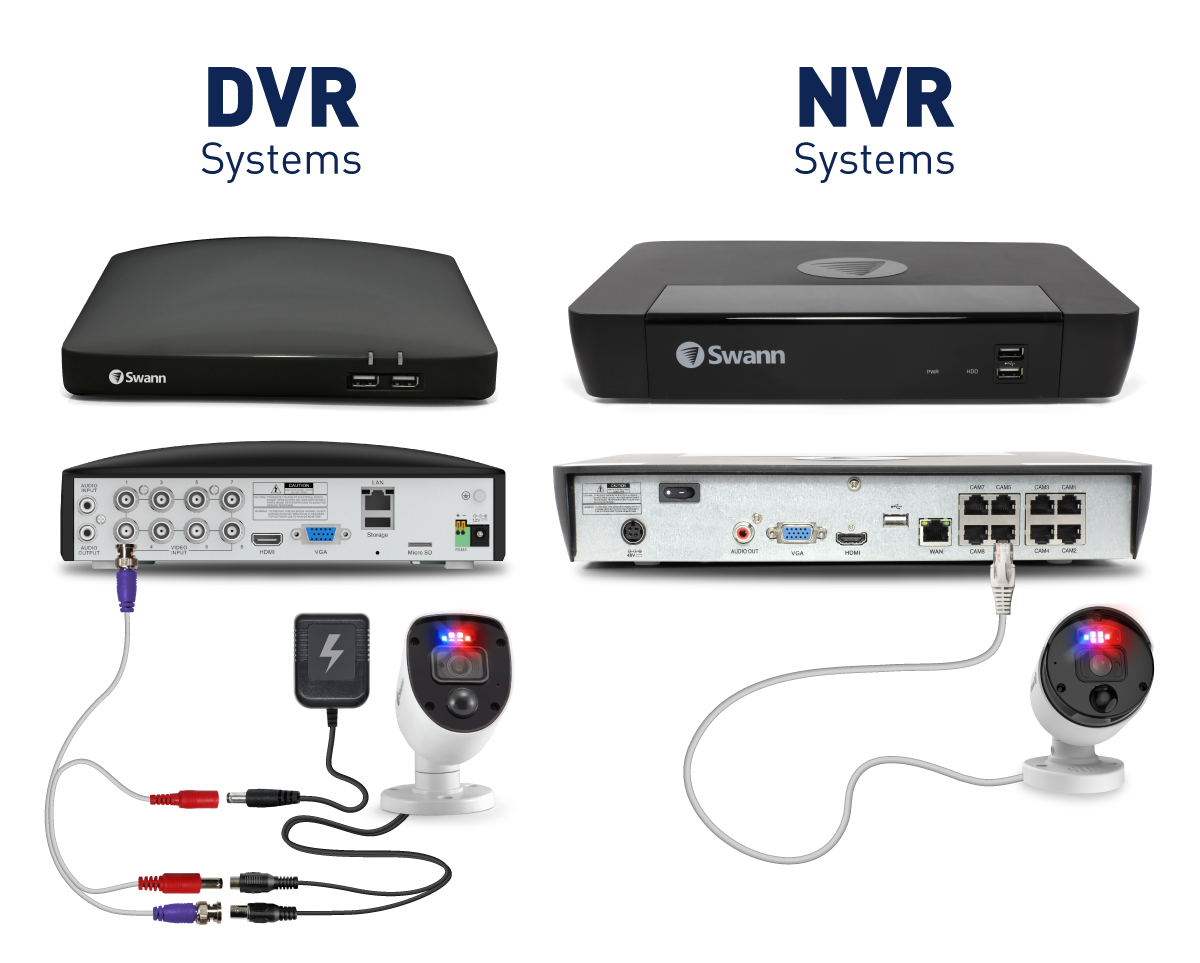
\includegraphics[width=0.7\textwidth]{casestudy/DVR.png}
\caption{Traditional DVR/NVR surveillance system}
\label{fig:dvr_system}
\end{figure}

\textbf{(B) Milestone XProtect:}
\hspace{0.8cm}Milestone XProtect sits at the other extreme — enterprise-grade, feature-rich, and priced accordingly. Multi-site management, detailed access controls, third-party analytics integrations. But it runs on Windows server infrastructure, charges per camera for licensing, and requires dedicated IT resources to maintain. For smaller organizations or individual users, it's simply out of reach, and even for larger ones the total cost of ownership is substantial.

\begin{figure}[H]
\centering
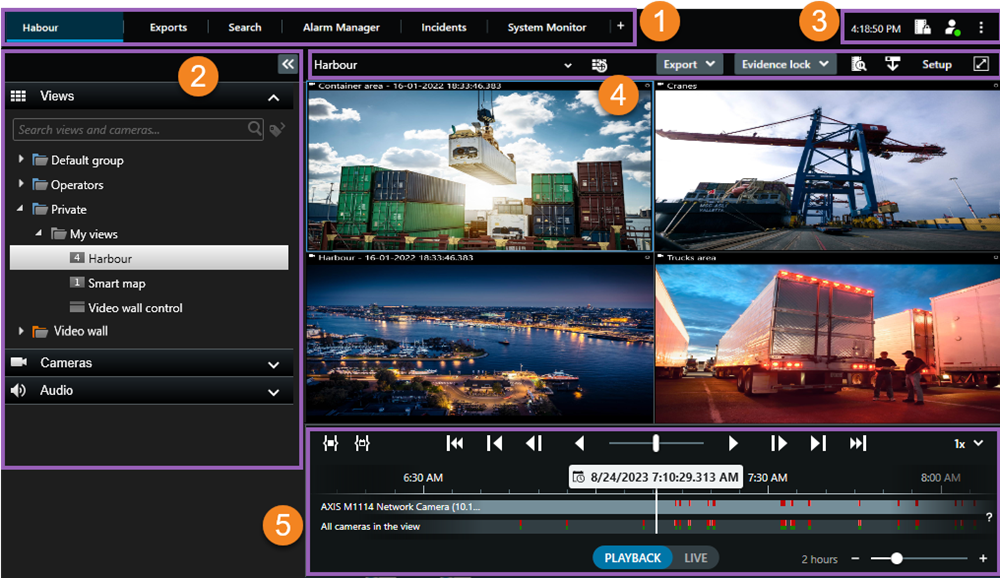
\includegraphics[width=0.7\textwidth]{casestudy/milestone.png}
\caption{The Milestone XProtect interface}
\label{fig:milestone}
\end{figure}

\textbf{(C) Frigate NVR:}
\hspace{0.8cm}Frigate was the most interesting case for us, because it's genuinely powerful for what it is. Open-source, AI-powered detection, great Home Assistant integration. We spent a few hours setting it up during the research phase and we were impressed. But the configuration complexity is real — you need to know what you're doing with YAML files, Docker networking, and hardware acceleration. And there's no collaborative sharing model at all. It's very much a tool for the technically inclined individual, not for an organization that needs to manage access for multiple people.

\begin{figure}[H]
\centering
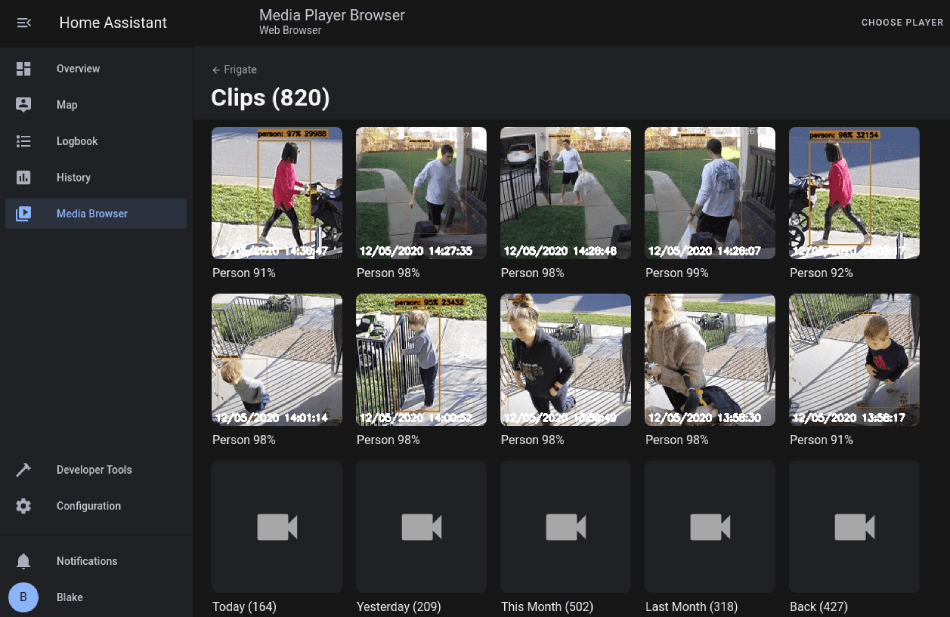
\includegraphics[width=0.7\textwidth]{casestudy/frigate.png}
\caption{The Frigate NVR interface}
\label{fig:frigate}
\end{figure}

\subsubsection{Criticism of the Existing System}
\hspace{0.8cm}After looking at all three, some patterns became obvious:
\begin{itemize}
  \item \textbf{Vendor Lock-in:} Commercial platforms tie you to their hardware or their cloud, making it expensive and painful to switch when your needs change.
  \item \textbf{Limited Remote Access:} Getting reliable remote viewing typically means opening ports and configuring VPNs, which introduces security risks most users aren't equipped to manage.
  \item \textbf{No Collaborative Sharing:} None of the platforms we evaluated natively supports sharing camera access with specific users through a proper permission-based system. It's either everyone or nobody.
  \item \textbf{Rigid Storage Options:} You're usually committed to one storage backend. Switching means migrating everything.
  \item \textbf{High Configuration Barrier:} Open-source tools require serious technical knowledge to deploy. That's fine for experts, but it excludes a massive potential audience.
  \item \textbf{No Detection Zones:} Very few platforms let you draw custom monitoring regions on a live feed, assign severity levels, and schedule when those zones should be active.
\end{itemize}

\subsubsection{Project Goals}
\hspace{0.8cm}Based on everything we'd seen, we set out the following targets for VigileEye:
\begin{itemize}
  \item A web-based platform for centralized IP camera management supporting RTSP, HTTP, RTMP, ONVIF, and HLS.
  \item A solid authentication stack combining JWT sessions, two-factor authentication via email OTP, and Google OAuth.
  \item Collaborative camera sharing through an invitation-based system with role-based permissions and group management.
  \item Real-time video via WebRTC targeting sub-second latency, with HTTP JPEG polling as an automatic fallback when WebRTC can't complete negotiation.
  \item A storage system that can write recordings to a local filesystem, MinIO, or Azure Blob Storage, switchable per camera, with configurable retention policies.
  \item Polygon-based detection zones with scheduling and severity-level alerting.
  \item Clean Architecture across all microservices to keep business logic decoupled from infrastructure.
  \item A React Native mobile app covering both iOS and Android.
\end{itemize}

\subsubsection{Solution Overview}
\hspace{0.8cm}We built the platform as five independent microservices, each with a specific job. The \textbf{Authentication Service} handles everything identity-related: registration, email verification, two-factor authentication, Google OAuth, password management, and the full JWT token lifecycle. The \textbf{Members Service} owns the sharing layer — individual invitations, group creation, bulk invitations, and permission management.

\hspace{0.8cm}The \textbf{Camera Management Service} manages each camera's full lifecycle: creation, configuration, health monitoring, and detection zone management with scheduling. The \textbf{Streaming Service}, written in Go, ingests RTSP streams via FFmpeg, pushes them to MediaMTX, and serves WebRTC feeds to viewers using the WHEP protocol. The \textbf{Storage Service}, also in Go, manages segmented MP4 recording using the Strategy Pattern to abstract the storage backend completely. On the frontend, a React/TypeScript SPA acts as the control center for the entire system, backed by a React Native mobile companion.

% ────────────────────────────────────────────────────────────────────────
\subsection{Investigation of Approaches}
\label{subsec:methodology_study}

\hspace{0.8cm}We didn't just jump straight into coding. Picking the right methodology was actually a real conversation between us, because the wrong choice could have derailed the whole project. We looked at three agile frameworks and measured them against what we actually needed.

\subsubsection{Agile Methodology: Scrum}
\hspace{0.8cm}Scrum is built around short, time-boxed iterations called sprints — usually one to four weeks — each ending with something you can actually show someone. Three roles: Product Owner, Scrum Master, Development Team. Four ceremonies: sprint planning, daily standup, sprint review, retrospective. The structure sounds simple, but it creates a discipline that keeps the team honest about what's been done and what still needs attention. Blockers surface early. Goals stay visible. Scope creep has to fight against a defined sprint boundary to get in.

\begin{figure}[H]
\centering
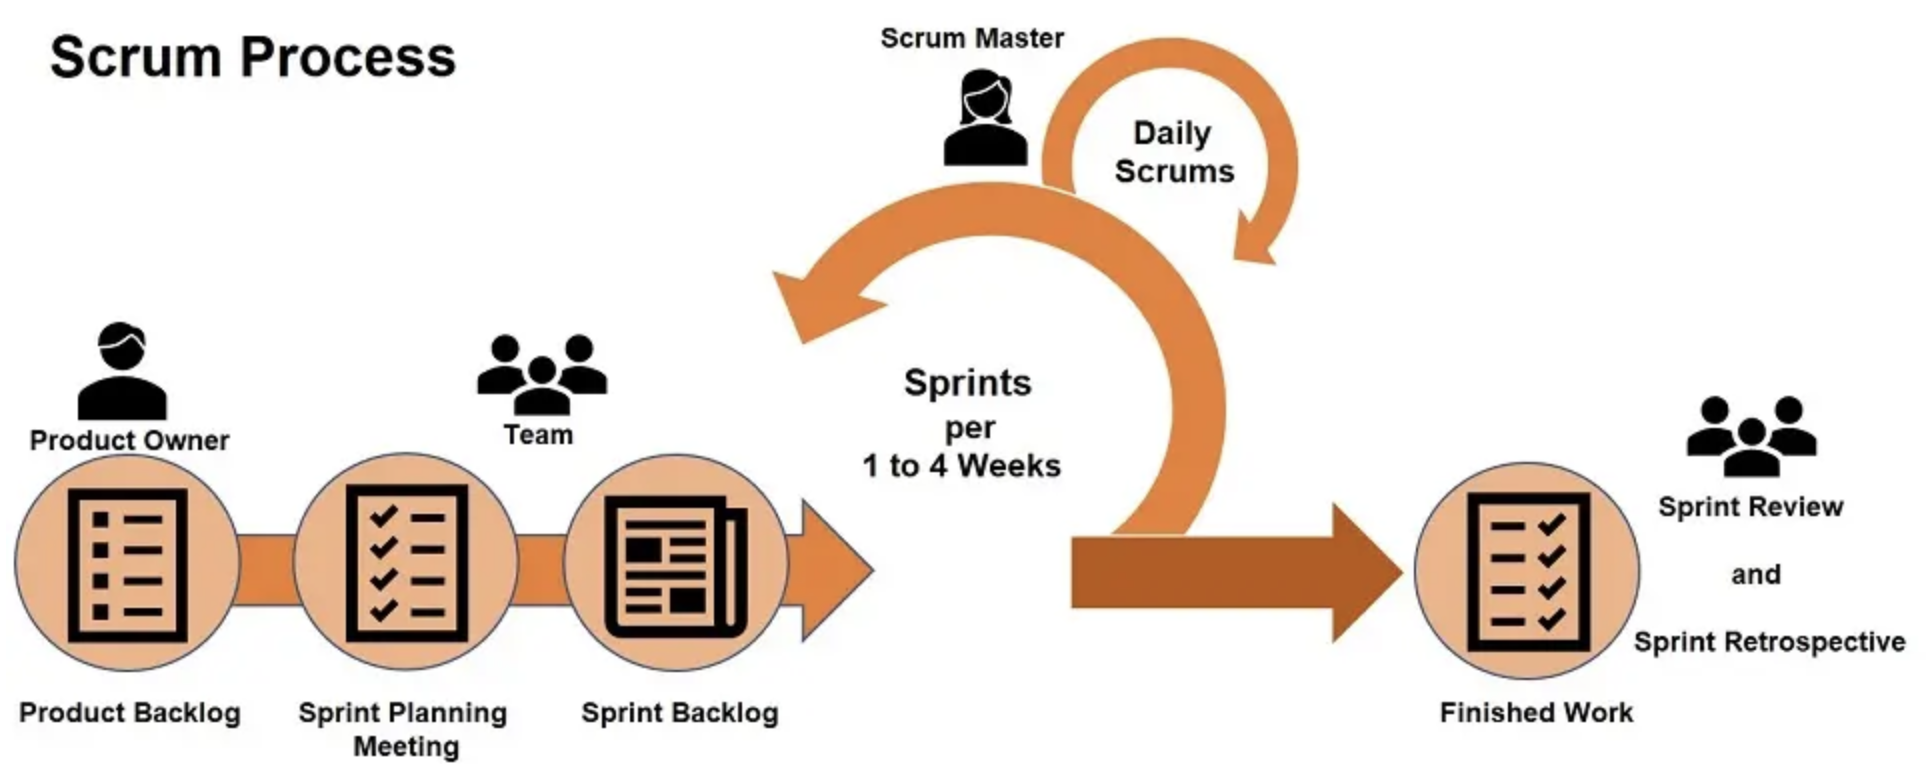
\includegraphics[width=0.9\textwidth]{casestudy/scrum.png}
\caption{SCRUM methodology cycle}
\label{fig:scrum_cycle}
\end{figure}

\subsubsection{Methodology Comparison: Scrum, XP, and Kanban}
\hspace{0.8cm}Table~\ref{tab:methodology_comparison} summarizes how Scrum, Extreme Programming, and Kanban stack up against the dimensions that mattered most for VigileEye.

\begin{longtable}{|>{\bfseries\small}p{3.2cm}|p{3.5cm}|p{3.5cm}|p{3.5cm}|}
\hline
\rowcolor{gray!20}
\textbf{Criterion} & \textbf{Scrum} & \textbf{Extreme Programming (XP)} & \textbf{Kanban} \\
\hline
\endfirsthead
\hline
\rowcolor{gray!20}
\textbf{Criterion} & \textbf{Scrum} & \textbf{Extreme Programming (XP)} & \textbf{Kanban} \\
\hline
\endhead
\hline
\endfoot
Iteration Model & Fixed-length sprints (1--4 weeks) with defined goals & Short release cycles, continuous integration & Continuous flow, no fixed iterations \\
\hline
Team Roles & Defined roles: Product Owner, Scrum Master, Team & No explicit role separation & No predefined roles \\
\hline
Planning & Sprint planning, backlog grooming, sprint review & Release planning and iteration planning & Just-in-time planning \\
\hline
Deliverables & Working increment at end of each sprint & Frequent small releases & Continuous delivery of tasks \\
\hline
Feedback & Sprint reviews and retrospectives & Pair programming, test-driven development & Implicit through WIP limits \\
\hline
Adaptability & Adapts at sprint boundaries & Adapts through continuous testing and refactoring & Highly adaptive, changes anytime \\
\hline
Suitability & Complex projects with evolving requirements and multiple stakeholders & Technically demanding projects with strong engineering discipline & Ongoing maintenance or support workflows \\
\hline
Transparency & High -- via backlog, sprint board, and burndown charts & Moderate & Moderate -- via Kanban board \\
\hline
Best Fit for VigileEye & \textbf{Excellent} -- microservices with vertical slices per sprint & Partial -- lacks structured delivery milestones & Not ideal -- project requires clear sprint goals \\
\hline
\caption{Comparative Analysis of Agile Methodologies}
\label{tab:methodology_comparison}
\end{longtable}

\subsubsection{Why Scrum}
\hspace{0.8cm}The comparison made it pretty clear. VigileEye spans five microservices in two different languages, and the requirements evolved as we learned more about what WebRTC and the storage subsystem actually needed in practice. Scrum's sprint structure let us carve the backlog into meaningful chunks — one service domain per sprint — so at the end of each iteration we had something concrete to demo rather than a half-finished pile of infrastructure. Kanban's continuous-flow model would have blurred the boundaries between phases and made it impossible to set honest expectations with our supervisor. XP has good engineering practices, but it doesn't give you the backlog structure and role clarity needed to coordinate a multi-service project with an external stakeholder. Scrum hit the right balance for what we were doing.

\subsubsection{Project Management with Jira}
\hspace{0.8cm}We used Jira throughout the project to manage sprints, track user stories, and keep tabs on individual tasks. Beyond basic tracking, the velocity charts and burndown diagrams gave us an honest picture of our real pace — which, at a couple of points in Sprint II, was a useful reality check. Spotting that we were falling behind on the streaming service mid-sprint gave us time to adjust priorities before it became a real problem.

\begin{figure}[H]
\centering

\includegraphics[width=0.3\textwidth]{Tech/jira.png}
\caption{Jira logo}
\label{fig:jira_logo}
\end{figure}

\subsubsection{Version Control with GitHub}
\hspace{0.8cm}Every microservice had its own GitHub repository with a consistent branching strategy: a protected \texttt{main} branch, a shared \texttt{develop} branch, and feature branches named after user story IDs. Pull requests were mandatory before anything merged into \texttt{develop} — no exceptions. This kept the shared branch stable and meant we always had a second pair of eyes on the code before it became official. There were definitely a few times where a code review caught something that would have caused real pain later.

\begin{figure}[H]
\centering

\includegraphics[width=0.3\textwidth]{Tech/github.png}
\caption{GitHub logo}
\label{fig:github_logo}
\end{figure}

\subsection*{Conclusion}

\hspace{0.8cm}This first part grounded the project in its professional context, introduced the organization we worked with, and made the case for why existing surveillance tools weren't good enough. From that foundation we defined what VigileEye needed to achieve. The methodology comparison led us to Scrum — not by default, but because it genuinely fit the nature of what we were building better than the alternatives.

% ════════════════════════════════════════════════════════════════════════
\newpage
\section{Requirements Analysis and Specifications}
\label{sec:requirements}
% ════════════════════════════════════════════════════════════════════════

\subsection*{Introduction}

\hspace{0.8cm}With context established, this second part gets into the specifics. Who uses the system? What do they need it to do? What constraints apply to how it does those things? We work through actors, functional requirements, non-functional quality attributes, and then move into technology choices backed by actual comparative data. The architecture decisions follow from those choices, and the part closes with the product backlog, sprint planning, and timeline.

% ────────────────────────────────────────────────────────────────────────
\subsection{Requirements Analysis}
\label{subsec:requirements_analysis}

\subsubsection{Actors Identification}
\hspace{0.8cm}Four distinct types of users interact with VigileEye, each with different needs and permissions.

\textbf{(A) Camera Owner:} The central user of the platform. Camera Owners register cameras, set up detection zones, start streaming and recording sessions, manage storage settings, and invite other users to share access. They have full administrative control over their surveillance infrastructure.

\textbf{(B) Invited Member (Reader):} A user who has received and accepted a sharing invitation. Readers can watch live feeds, browse recordings, and check camera status — but they can't touch any configuration settings.

\textbf{(C) Invited Member (Editor):} An invited user with elevated rights. Editors can do everything a Reader can, plus modify camera settings, manage detection zones, and control recording sessions for cameras they've been granted access to.

\textbf{(D) Group Member:} A user belonging to a sharing group created by a Camera Owner. Group members inherit whatever permission level the group was set up with and get access to all cameras associated with that group.

\subsubsection{Static Context Diagram}
\hspace{0.8cm}The static context diagram below shows VigileEye at a high level, illustrating how it interacts with external actors and systems.

\begin{figure}[H]
\centering
\fbox{\parbox{12cm}{\centering\vspace{3cm}Static Context Diagram\vspace{3cm}}}
\caption{Static Context Diagram}
\label{fig:context_diagram}
\end{figure}

\subsubsection{Functional Requirements}
\hspace{0.8cm}Table~\ref{tab:functional_requirements} lists the functional requirements grouped by actor.

\begin{longtable}{|>{\bfseries\small}p{3cm}|p{10.5cm}|}
\hline
\textbf{Actor} & \textbf{Requirements} \\
\hline
\endfirsthead
\hline
\textbf{Actor} & \textbf{Requirements} \\
\hline
\endhead
\hline
\endfoot
Camera Owner &
\begin{itemize}[nosep,leftmargin=1em]
  \item Register an account with email and password.
  \item Verify email using a one-time passcode.
  \item Log in with two-factor authentication (email OTP).
  \item Log in using Google OAuth.
  \item Request and complete password reset.
  \item View login history with device, IP, and location details.
  \item Create, update, delete, enable, and disable cameras.
  \item Configure camera details (resolution, FPS, encoding, location).
  \item View camera health metrics (latency, frame drops, uptime).
  \item Create, update, activate, deactivate, and delete detection zones.
  \item Configure zone scheduling and alert severity.
  \item Start and stop live camera streams.
  \item View live streams via WebRTC or HTTP polling fallback.
  \item Start, stop, and manage recording sessions.
  \item Configure storage settings (backend, retention, quality).
  \item View storage metrics and manage subscription tier.
  \item Send camera-sharing invitations to other users.
  \item Create and manage sharing groups with bulk invitation support.
\end{itemize} \\
\hline
Invited Member &
\begin{itemize}[nosep,leftmargin=1em]
  \item Register and authenticate using the same mechanisms as the Camera Owner.
  \item View received invitations and accept or decline them using approval codes.
  \item View shared camera feeds via live streaming.
  \item Browse recordings of shared cameras.
  \item Modify camera settings when editor-level permission has been granted.
\end{itemize} \\
\hline
\caption{Functional Requirements by Actor}
\label{tab:functional_requirements}
\end{longtable}

\subsubsection{Non-Functional Requirements}
\hspace{0.8cm}Beyond what the system does, there are constraints on how well it has to do it. These weren't negotiable.

\textbf{Security:} All access is gated through JWT tokens combined with two-factor authentication and Google OAuth. Passwords are hashed using bcrypt with twelve salt rounds — not ten, twelve, because we checked and it was worth the extra millisecond. After three failed login attempts, accounts get locked for an hour. Role-based access control makes sure that invited members can't do things they were never given permission to do.

\textbf{Performance:} The platform targets sub-second end-to-end latency for live WebRTC streams served through MediaMTX. HTTP JPEG polling provides a configurable-interval fallback when WebRTC negotiation can't complete — important for users behind restrictive firewalls or double NAT.

\textbf{Ergonomics:} The React frontend is fully responsive across desktops, tablets, and phones. The React Native app provides a native feel on iOS and Android, so monitoring doesn't have to happen at a desk.

\textbf{Scalability:} Every microservice can scale horizontally in isolation. The storage service uses the Strategy Pattern specifically so that the backend can be changed per camera without touching any recording logic.

\textbf{Reliability:} Retention policies run automatically so storage doesn't silently fill up. Camera health monitoring catches connectivity problems proactively. When WebRTC fails, the system degrades to HTTP polling instead of showing a blank screen.

% ────────────────────────────────────────────────────────────────────────
\subsection{Technical Specifications}
\label{subsec:technical_specs}

\subsubsection{Hardware Environment}
\hspace{0.8cm}We developed on two machines. One was Mohamed Yassin's MacBook Pro M1 Pro, which handled most of the iOS-side React Native work and ran the Python services with ease. Omar worked on a Lenovo IdeaPad Gaming 3, which had the GPU headroom for FFmpeg processing and ran the Go streaming benchmarks without breaking a sweat.

\begin{table}[H]
\centering
\begin{tabular}{|l|l|c|}
\hline
\textbf{Component} & \textbf{Specification} & \textbf{Image} \\
\hline
Computer           & MacBook Pro 14'' M1 Pro         & \multirow{6}{*}{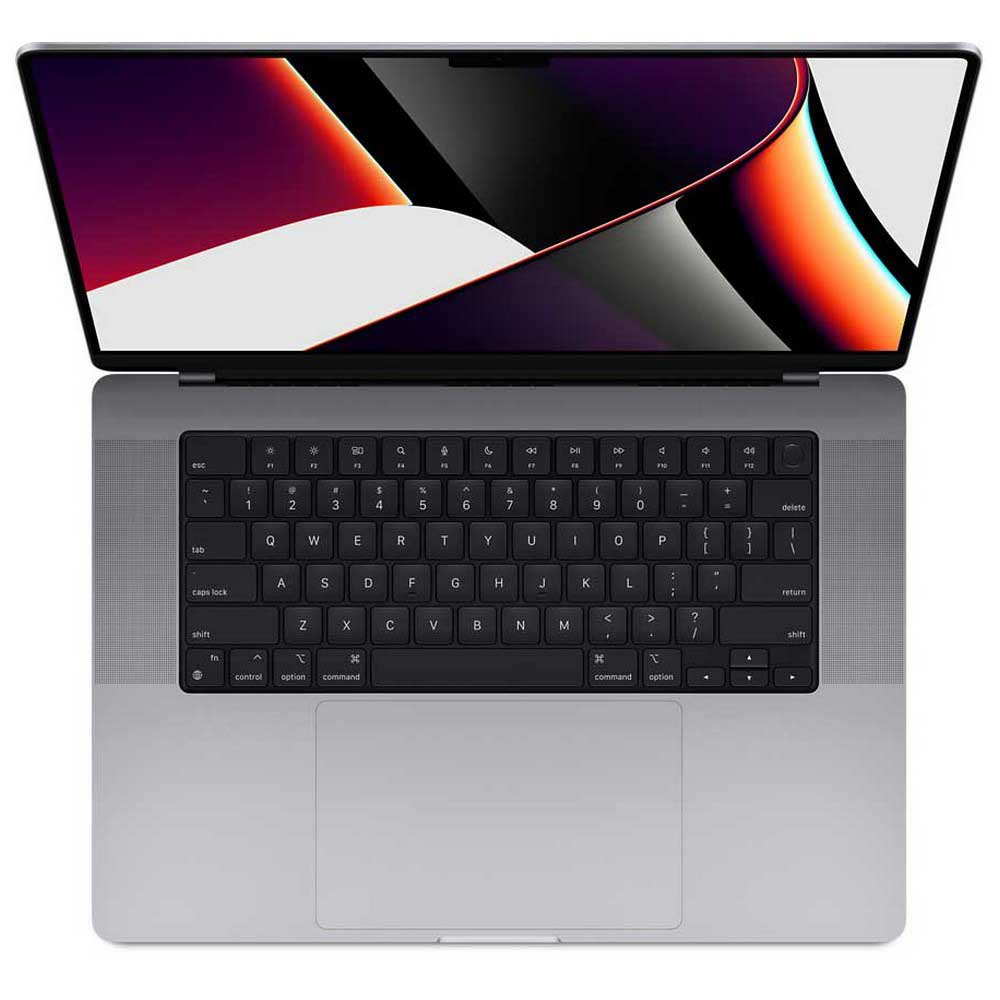
\includegraphics[width=3cm]{Machines/mac.png}} \\ \cline{1-2}
Operating System   & macOS Tahoe 26                 & \\ \cline{1-2}
Processor          & Apple M1 Pro 10-core CPU       & \\ \cline{1-2}
Graphics Card      & Apple 16-core GPU              & \\ \cline{1-2}
RAM                & 16 GB Unified Memory           & \\ \cline{1-2}
Storage            & 512 GB SSD                     & \\ \hline
\end{tabular}
\caption{Hardware Specifications of MacBook Pro M1 Pro}
\label{tab:mac_hardware}
\end{table}

\begin{table}[H]
\centering
\begin{tabular}{|l|l|c|}
\hline
\textbf{Component} & \textbf{Specification} & \textbf{Image} \\
\hline
Computer           & Lenovo IdeaPad Gaming 3        & \multirow{6}{*}{
\includegraphics[width=3cm]{Machines/lenovo.png}} \\ \cline{1-2}
Operating System   & Windows 11 Home                & \\ \cline{1-2}
Processor          & AMD Ryzen 5 5600H 6-core CPU   & \\ \cline{1-2}
Graphics Card      & NVIDIA GeForce RTX 3060 6\,GB  & \\ \cline{1-2}
RAM                & 20 GB DDR4                     & \\ \cline{1-2}
Storage            & 512 GB SSD                     & \\ \hline
\end{tabular}
\caption{Hardware Specifications of Lenovo IdeaPad}
\label{tab:lenovo_hardware}
\end{table}

\subsubsection{Technological Environment}

\begin{longtable}{|>{\centering\arraybackslash}m{2.5cm}|m{5.5cm}|m{5.5cm}|}
\hline
\textbf{Logo} & \textbf{Description} & \textbf{Why?} \\
\hline
\endfirsthead
\hline \textbf{Logo} & \textbf{Description} & \textbf{Why?} \\ \hline
\endhead
\hline
\endfoot

\raisebox{-0.2\height}{
\includegraphics[width=2cm]{Tech/fastapi.png}}
  & FastAPI: high-performance Python web framework for building APIs with automatic OpenAPI documentation.
  & Asynchronous request handling via ASGI, built-in data validation through Pydantic, and auto-generated interactive docs that actually saved us time during testing. \\ \hline

\raisebox{-0.2\height}{
\includegraphics[width=2cm]{Tech/go.png}}
  & Go (Golang): statically typed, compiled language built for simplicity, reliability, and high-concurrency systems.
  & Native goroutine concurrency and compiled-level throughput make it ideal for managing thousands of simultaneous stream connections. No other language came close in our benchmarks. \\ \hline

\raisebox{-0.2\height}{
\includegraphics[width=2cm]{Tech/react.png}}
  & React: JavaScript library for building interactive user interfaces, particularly single-page applications.
  & Virtual DOM diffing keeps the UI responsive, and TypeScript support catches integration bugs at compile time rather than in production. \\ \hline

\raisebox{-0.2\height}{
\includegraphics[width=2cm]{Tech/react.png}}
  & React Native: cross-platform mobile framework producing iOS and Android apps from a shared codebase.
  & Sharing hooks and business logic with the web frontend cuts duplication substantially while still delivering near-native performance on mobile. \\ \hline

\raisebox{-0.2\height}{
\includegraphics[width=2cm]{Tech/typescript.png}}
  & TypeScript: typed superset of JavaScript providing static analysis and richer tooling.
  & Bugs that would only appear at runtime in plain JavaScript get caught during compilation — in a codebase this size, that matters a lot. \\ \hline

\raisebox{-0.2\height}{
\includegraphics[width=2cm]{Tech/postgresql.png}}
  & PostgreSQL: advanced open-source relational database, hosted on Neon for shared cloud access.
  & JSON column support, strong transactions, and Neon's branching feature let both of us share a live schema without ever overwriting each other's changes. \\ \hline

\raisebox{-0.2\height}{
\includegraphics[width=2cm]{Tech/sqlalchemy.png}}
  & SQLAlchemy: Python SQL toolkit and ORM library.
  & Provides a solid persistence layer for the Python-based services, with Alembic managing schema migrations declaratively so we never touched the database directly. \\ \hline

\raisebox{-0.2\height}{
\includegraphics[width=2cm]{Tech/ffmpeg.png}}
  & FFmpeg: cross-platform multimedia framework for recording, converting, and streaming audio and video.
  & Used for RTSP-to-RTP ingestion into MediaMTX, segmented MP4 recording, and single-frame JPEG extraction for the HTTP fallback path. Incredibly powerful once you understand the argument syntax. \\ \hline

\raisebox{-0.2\height}{
\includegraphics[width=2cm]{Tech/webrtc.png}}
  & WebRTC: open standard for real-time peer-to-peer media communication in browsers.
  & Eliminates plugin dependencies and achieves the sub-second latency that surveillance monitoring genuinely requires. \\ \hline

\raisebox{-0.2\height}{
\includegraphics[width=2cm]{Tech/mediamtx.png}}
  & MediaMTX: real-time media server supporting RTSP, WebRTC, HLS, and RTMP.
  & Acts as the central stream relay, handling WHIP/WHEP negotiation with browsers and keeping the Go service from having to deal with ICE complexity directly. \\ \hline

\raisebox{-0.2\height}{
\includegraphics[width=2cm]{Tech/aws.png}}
  & AWS / Azure: cloud platforms for scalable storage, compute, and networking.
  & Azure Blob Storage is one of the three selectable recording backends, offering durable geo-redundant object storage without self-hosted infrastructure. \\ \hline

\raisebox{-0.2\height}{
\includegraphics[width=2cm]{Tech/yolo.png}}
  & YOLO (You Only Look Once): real-time object detection system.
  & Single-pass architecture processes video frames fast enough to keep up with live feeds — the detection engine the zone alerting subsystem is designed to plug into. \\ \hline

\caption{Technological Environment}
\label{tab:tech_env}
\end{longtable}

\paragraph{Why FastAPI for the Authentication and Camera Management Services?}

\hspace{0.8cm}We looked at three Python frameworks seriously: FastAPI, Django REST Framework, and Flask. Here's how they compared across the things we actually cared about.

\begin{table}[H]
\centering
\begin{tabular}{|>{\bfseries\small}p{3.2cm}|p{3cm}|p{3.2cm}|p{3.2cm}|}
\hline
\rowcolor{gray!20}
\textbf{Criterion} & \textbf{FastAPI} & \textbf{Django REST} & \textbf{Flask} \\
\hline
Performance & \textbf{Excellent} -- async ASGI & Good -- WSGI, sync-heavy & Moderate -- micro, sync \\
\hline
Auto Validation & \textbf{Built-in} via Pydantic & Manual serializers & Manual, extra libs needed \\
\hline
API Documentation & \textbf{Auto-generated} (Swagger/ReDoc) & Third-party add-on & Manual integration \\
\hline
Type Safety & \textbf{Native} Python type hints & Partial & Partial \\
\hline
Clean Architecture Fit & \textbf{Excellent} -- lightweight, flexible DI & Complex -- heavy ORM coupling & Good but minimal \\
\hline
Learning Curve & \textbf{Low} -- Pythonic, intuitive & Moderate & Low \\
\hline
Async Support & \textbf{Native} async/await & Partial (Django 3.1+) & Limited \\
\hline
Microservices Fit & \textbf{Excellent} -- lightweight, fast startup & Overkill for microservices & Good but limited \\
\hline
\rowcolor{green!10}
\textbf{Best Choice} & \textbf{\checkmark Yes} & No & No \\
\hline
\end{tabular}
\caption{FastAPI vs.\ Django REST Framework vs.\ Flask -- Comparison for Auth \& Camera Management Services}
\label{tab:fastapi_comparison}
\end{table}

\paragraph{Why Go (Golang) for the Streaming and Storage Services?}

\hspace{0.8cm}Streaming and storage have a fundamentally different performance profile — they need to sustain thousands of concurrent connections with minimal latency and very low per-stream overhead. Go's compiled execution model and goroutine scheduler exist precisely for this kind of workload. We tested the numbers and the table below is the result. There was really no discussion after we saw them.

\begin{table}[H]
\centering
\begin{tabular}{|>{\bfseries\small}p{3.2cm}|p{3cm}|p{3.2cm}|p{3.2cm}|}
\hline
\rowcolor{gray!20}
\textbf{Criterion} & \textbf{Go (Golang)} & \textbf{Node.js} & \textbf{Python / FastAPI} \\
\hline
Concurrency Model & \textbf{Goroutines} -- native M:N threads & Single event loop & Asyncio -- limited parallelism \\
\hline
WebRTC Library & \textbf{pion/webrtc} -- mature, production-ready & wrtc -- limited community & Not production-grade \\
\hline
CPU Performance & \textbf{Compiled}, near-C speed & JIT-compiled, moderate & Interpreted, slowest \\
\hline
Memory Efficiency & \textbf{Excellent} -- low GC overhead & Good -- V8 GC overhead & Moderate \\
\hline
Real-Time Streaming & \textbf{Excellent} -- goroutines per stream & Good -- may bottleneck & Not ideal for high load \\
\hline
Strategy Pattern & \textbf{Clean} interfaces, idiomatic Go & Possible but verbose & Possible via ABCs \\
\hline
FFmpeg Integration & \textbf{Native} exec.Command, low overhead & child\_process, moderate overhead & subprocess, highest overhead \\
\hline
\rowcolor{green!10}
\textbf{Best Choice} & \textbf{\checkmark Yes} & No & No \\
\hline
\end{tabular}
\caption{Go vs.\ Node.js vs.\ Python/FastAPI -- Comparison for Streaming \& Storage Services}
\label{tab:go_comparison}
\end{table}

\paragraph{Streaming Performance: Go Alone vs.\ Go + MediaMTX}

\hspace{0.8cm}Early in the architecture phase, we ran a benchmark comparing a pure Go WebRTC implementation against our hybrid Go + MediaMTX stack. The numbers in Figure~\ref{fig:chart_go_mediamtx} explain why we went with the relay approach. Going from 420ms latency down to 120ms, and from 35 concurrent streams up to 120 — that's not a marginal improvement, that's a completely different capability level.

\begin{figure}[H]
\centering

\includegraphics[width=0.75\textwidth]{\detokenize{charts/streamingAllLang.png}}
\caption{Performance comparison: Go standalone vs.\ Go + MediaMTX}
\label{fig:chart_go_mediamtx}
\end{figure}

\paragraph{Streaming Framework Comparison: Go+MediaMTX vs.\ Node.js vs.\ FastAPI}

\hspace{0.8cm}We extended the benchmark to cover all three candidate stacks. Figure~\ref{fig:chart_streaming_compare} shows the results, and they were consistent with what we'd expected — but seeing them laid out like this removed any remaining doubt.

\begin{figure}[H]
\centering

\includegraphics[width=0.75\textwidth]{\detokenize{charts/Streamingwithout.png}}
\caption{Streaming stack comparison: Go+MediaMTX vs.\ Node.js vs.\ FastAPI}
\label{fig:chart_streaming_compare}
\end{figure}

\paragraph{Why React (and React Native) for the Frontend?}

\hspace{0.8cm}The decision between React/React Native and Flutter came down to three things: WebRTC browser API support, code reuse between web and mobile, and the fact that we both already knew React well. Dart was a learning overhead we simply couldn't afford within the project timeline.

\begin{table}[H]
\centering
\begin{tabular}{|>{\bfseries\small}p{3.4cm}|p{4.5cm}|p{4.5cm}|}
\hline
\rowcolor{gray!20}
\textbf{Criterion} & \textbf{React + React Native} & \textbf{Flutter} \\
\hline
Language & JavaScript / TypeScript -- widely adopted & Dart -- smaller ecosystem \\
\hline
Web + Mobile & \textbf{Shared codebase} between React (web) and React Native (mobile) & Separate rendering engine for web, still maturing \\
\hline
Ecosystem & \textbf{Largest} -- npm, millions of packages & Growing but considerably smaller \\
\hline
WebRTC Support & \textbf{Native} browser APIs + react-webrtc & Plugin-based, limited \\
\hline
TypeScript Integration & \textbf{First-class} support & Not applicable (Dart) \\
\hline
Component Reuse & \textbf{High} -- hooks and logic shared across web and mobile & Moderate -- widget-based, not shared with web \\
\hline
MVVM Pattern & \textbf{Excellent} -- custom hooks as ViewModels & Possible but non-idiomatic \\
\hline
Team Expertise & \textbf{High} -- both developers proficient in React & Low -- Dart learning overhead \\
\hline
Community Support & \textbf{Largest} in frontend development & Growing, smaller \\
\hline
Production Maturity & \textbf{Extremely mature} -- used by Meta, Netflix & Mature for mobile, less so for web \\
\hline
\rowcolor{green!10}
\textbf{Best Choice} & \textbf{\checkmark Yes} & No \\
\hline
\end{tabular}
\caption{React + React Native vs.\ Flutter -- Frontend Technology Comparison}
\label{tab:react_flutter}
\end{table}

\subsubsection{Software Environment}

\begin{longtable}{|>{\centering\arraybackslash}m{2.5cm}|m{5.5cm}|m{5.5cm}|}
\hline
\textbf{Logo} & \textbf{Description} & \textbf{Why?} \\
\hline
\endfirsthead
\hline \textbf{Logo} & \textbf{Description} & \textbf{Why?} \\ \hline
\endhead
\hline
\endfoot

\raisebox{-0.2\height}{
\includegraphics[width=2cm]{Tech/vscode.png}}
  & Visual Studio Code: lightweight, highly extensible source code editor.
  & Excellent support for Python, Go, TypeScript, and React through a rich extension marketplace. We practically lived in it. \\ \hline

\raisebox{-0.2\height}{
\includegraphics[width=2cm]{Tech/postman.png}}
  & Postman: API platform for designing, testing, and documenting HTTP interfaces.
  & Simplified manual and automated testing of REST endpoints across all five microservices. Collections made it easy to share test suites. \\ \hline

\raisebox{-0.2\height}{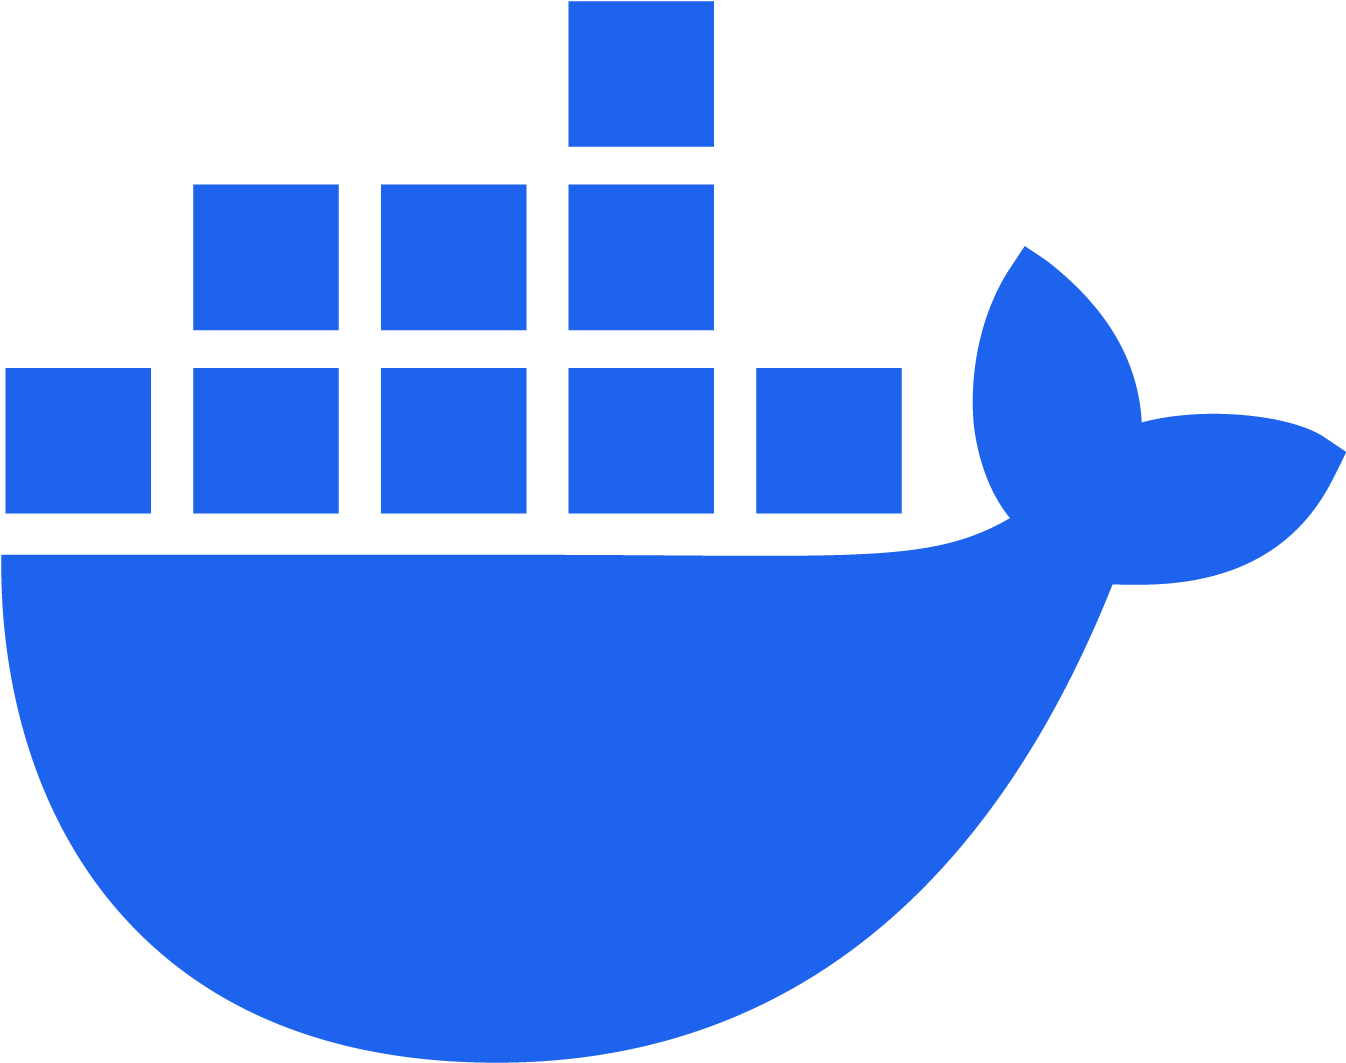
\includegraphics[width=2cm]{Tech/docker.png}}
  & Docker: container platform for packaging applications with all their dependencies.
  & Ensured a consistent runtime environment across both machines and made microservice orchestration straightforward. \\ \hline

\raisebox{-0.2\height}{
\includegraphics[width=2cm]{Tech/pgadmin.png}}
  & pgAdmin: open-source GUI for PostgreSQL administration.
  & Gave us a visual interface for schema inspection, query execution, and data verification during development — much faster than raw SQL in a terminal. \\ \hline

\raisebox{-0.2\height}{
\includegraphics[width=2cm]{Tech/overleaf.png}}
  & Overleaf: collaborative online \LaTeX\ editor.
  & Used for writing and formatting this report, enabling real-time collaboration between both authors without version conflicts. \\ \hline

\raisebox{-0.2\height}{
\includegraphics[width=2cm]{Tech/drawio.png}}
  & DrawIO: diagramming tool for system architecture and UML diagrams.
  & Produced all UML diagrams, architecture drawings, and workflow charts included in this report. \\ \hline

\raisebox{-0.2\height}{
\includegraphics[width=2cm]{Tech/xcode.png}}
  & Xcode: Apple's official IDE for iOS development.
  & Required for building and testing the iOS target of the React Native application on a physical device. \\ \hline

\raisebox{-0.2\height}{
\includegraphics[width=2cm]{Tech/jira.png}}
  & Jira: project management and issue tracking tool.
  & Used for sprint planning, backlog refinement, and daily task tracking throughout the project. \\ \hline

\raisebox{-0.2\height}{
\includegraphics[width=2cm]{Tech/notion.png}}
  & Notion: note-taking and organization workspace.
  & Helped document architectural decisions, record research findings, and plan feature designs before implementation. Very useful for keeping track of things across two developers. \\ \hline

\caption{Software Environment}
\label{tab:software_env}
\end{longtable}

\subsubsection{Additional Tools}

\hspace{0.8cm}\textbf{Git Workflow:} We followed a feature-branch workflow across all repositories. Every user story got its own branch off \texttt{develop}. Pull requests triggered peer review before any merge — nothing reached the shared branch without a second set of eyes. It sounds like overhead, but it caught actual bugs more than once.

\begin{figure}[H]
\centering
\fbox{\parbox{10cm}{\centering\vspace{2cm}Git Workflow Diagram\vspace{2cm}}}
\caption{Git Workflow}
\label{fig:git_workflow}
\end{figure}

\begin{table}[H]
\centering
\begin{tabular}{|l|p{8cm}|}
\hline
\textbf{Command} & \textbf{Description} \\ \hline
\texttt{git init}        & Initializes a new local Git repository \\ \hline
\texttt{git clone}       & Creates a local copy of a remote repository \\ \hline
\texttt{git commit -m}   & Records staged changes with a descriptive message \\ \hline
\texttt{git push}        & Uploads local branch changes to the remote repository \\ \hline
\texttt{git pull}        & Fetches and merges the latest changes from the remote \\ \hline
\texttt{git checkout -b} & Creates and switches to a new branch \\ \hline
\texttt{git merge}       & Integrates changes from one branch into another \\ \hline
\texttt{git status}      & Shows the current state of the working directory \\ \hline
\end{tabular}
\caption{Git Commands}
\label{tab:git_commands}
\end{table}

% ────────────────────────────────────────────────────────────────────────
\subsection{Project Architecture}
\label{subsec:architecture}

\hspace{0.8cm}Three architectural patterns govern VigileEye at different levels. Clean Architecture runs at the service level — keeping business logic completely isolated from whatever framework or database sits underneath. MVVM organizes the React frontend. And a microservices pattern structures the system as a whole. Each was chosen to solve a specific problem, not because it sounded good in a slide.

\subsubsection{Clean Architecture}
\hspace{0.8cm}Robert C.\ Martin's Clean Architecture organizes a codebase into concentric layers where dependencies only flow inward. Outer layers depend on inner ones, never the reverse. We applied this to every backend service with four distinct rings.

\textbf{Domain Layer (innermost):} Pure business logic — entities, value objects, repository interfaces, domain service interfaces. No framework import has any business being here.

\textbf{Application Layer:} Use cases that orchestrate domain objects to fulfill specific user intentions, plus DTOs that decouple the API's representation from the internal model.

\textbf{Infrastructure Layer:} Concrete implementations of the inner-layer interfaces — SQLAlchemy repositories for Python services, Go repository implementations, SMTP integrations, JWT tooling, bcrypt hashing.

\textbf{API Layer (outermost):} FastAPI route handlers or Gin HTTP handlers that parse requests, call use cases through injected dependencies, and serialize responses.

\begin{figure}[H]
\centering
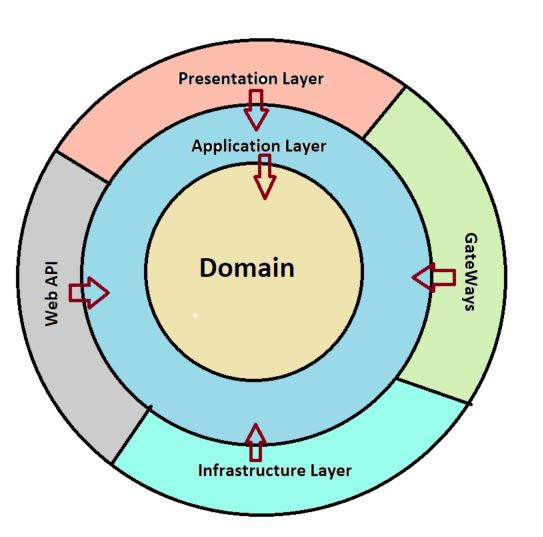
\includegraphics[width=0.5\textwidth]{Architecture/CleanArchitecture.jpeg}
\caption{Clean Architecture pattern}
\label{fig:clean_arch}
\end{figure}

\subsubsection{Microservices Architecture}
\hspace{0.8cm}VigileEye runs as five independent services, each owning its own PostgreSQL schema, deployed separately, exposing a well-defined REST API. Inter-service communication works by forwarding JWT tokens on HTTP calls — authentication logic stays centralized in the Auth service without creating any shared library dependency that would couple the services at build time. Hosting everything on Neon meant we were both hitting the same live database throughout development, which sounds like a minor detail until you realize how many environment-drift bugs it prevented.

\begin{figure}[H]
\centering
\fbox{\parbox{11cm}{\centering\vspace{3cm}Microservices Architecture Diagram\vspace{3cm}}}
\caption{VigileEye Microservices Architecture}
\label{fig:microservices}
\end{figure}

\subsubsection{Frontend Architecture: MVVM}
\hspace{0.8cm}The React frontend is organized around Model--View--ViewModel. The \textbf{Model} consists of TypeScript interfaces and API service modules that execute HTTP requests. The \textbf{View} is React components rendering JSX, styled with Tailwind CSS. The \textbf{ViewModel} is custom hooks like \texttt{useAllCameras}, \texttt{useWebRTCStream}, \texttt{useWHEPStream}, and \texttt{useAudioStream} that manage state, side effects, and the WebRTC connection lifecycle — including the automatic fallback to HTTP polling when WebRTC can't connect.

\begin{figure}[H]
\centering
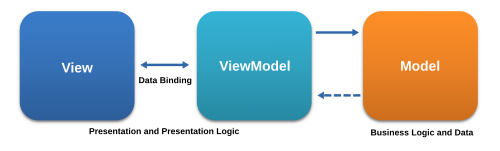
\includegraphics[width=0.8\textwidth]{Architecture/mvvm.png}
\caption{MVVM Architecture Pattern (React Frontend)}
\label{fig:mvvm}
\end{figure}

\subsubsection{Backend Service Architectures}

\textbf{FastAPI Services (Auth \& Camera Management):} Both Python services use FastAPI with SQLAlchemy ORM, Alembic for schema migrations, and Pydantic for request validation. FastAPI's dependency injection maps naturally onto Clean Architecture's ports-and-adapters concept, which made wiring everything together feel almost natural.

\textbf{Go Services (Streaming \& Storage):} The Go services use the Gin HTTP framework. The Streaming service coordinates FFmpeg as the camera ingestor, MediaMTX as the stream relay, and the \texttt{pion/webrtc} library for WebRTC negotiation. The Storage service uses the Strategy Pattern to swap between LocalFS, MinIO, and Azure Blob backends, while goroutines manage concurrent recording sessions without any blocking.

\subsubsection{Overall Application Structure}

\begin{figure}[H]
\centering
\fbox{\parbox{12cm}{\centering\vspace{3.5cm}Overall Application Architecture Diagram\vspace{3.5cm}}}
\caption{General architecture of the VigileEye application}
\label{fig:overall_arch}
\end{figure}

% ────────────────────────────────────────────────────────────────────────
\subsection{Scrum Methodology in Project Management}
\label{subsec:scrum_mgmt}

\hspace{0.8cm}At the start of the project, the Product Owner — our supervisor at IBSOFT — helped us populate the initial Product Backlog: an ordered list of everything the system needed to do. Three concepts governed how we managed it:
\begin{itemize}
  \item \textbf{Identifier:} A unique code assigned to each User Story for traceability.
  \item \textbf{User Story:} A short, plain-language statement describing a desired outcome from the perspective of a specific user.
  \item \textbf{Priority:} An importance ranking based on business value and delivery timeline.
\end{itemize}

% ────────────────────────────────────────────────────────────────────────
\subsection{Product Backlog}
\label{subsec:product_backlog}

\begin{longtable}{|>{\small}c|>{\small}p{2.5cm}|>{\small}p{7.2cm}|>{\small}c|}
\hline
\textbf{ID} & \textbf{Feature} & \textbf{User Story} & \textbf{Priority} \\
\hline
\endfirsthead
\hline \textbf{ID} & \textbf{Feature} & \textbf{User Story} & \textbf{Priority} \\ \hline
\endhead \hline
\endfoot \hline
\endlastfoot

1  & User Registration  & As a User, I want to register an account with email and password & High \\ \hline
   &                    & As a User, I want to verify my email using an OTP code & High \\ \hline
   &                    & As a User, I want to receive a 6-digit verification code via email & High \\ \hline
2  & User Authentication & As a User, I want to log in using email and password & High \\ \hline
   &                    & As a User, I want to receive a 2FA OTP code after entering credentials & High \\ \hline
   &                    & As a User, I want to confirm login with OTP & High \\ \hline
   &                    & As a User, I want to receive JWT access and refresh tokens & High \\ \hline
3  & Google OAuth       & As a User, I want to log in using my Google account & High \\ \hline
   &                    & As a User, I want to be redirected to Google's auth page & High \\ \hline
   &                    & As a User, I want auto-account creation for first-time Google login & High \\ \hline
4  & Password Mgmt      & As a User, I want to request a password reset & High \\ \hline
   &                    & As a User, I want to receive a reset OTP via email & High \\ \hline
   &                    & As a User, I want to set a new password after verifying OTP & High \\ \hline
5  & Token Mgmt         & As a User, I want auto-refresh of access tokens & High \\ \hline
   &                    & As a User, I want expired sessions handled gracefully & High \\ \hline
6  & Login History      & As a User, I want to view my login history & Medium \\ \hline
   &                    & As a User, I want details (IP, device, browser, OS, location) & Medium \\ \hline
   &                    & As a User, I want to filter history and view suspicious logins & Medium \\ \hline
7  & Invitation Mgmt    & As a Camera Owner, I want to invite users to share cameras & High \\ \hline
   &                    & As a Camera Owner, I want to specify permission level & High \\ \hline
   &                    & As a Camera Owner, I want invitation codes sent via email & High \\ \hline
8  & Invitation Track   & As a Camera Owner, I want to view sent invitations & High \\ \hline
   &                    & As a Camera Owner, I want to resend invitation codes & Medium \\ \hline
9  & Membership Mgmt    & As an Invited Member, I want to view received invitations & High \\ \hline
   &                    & As an Invited Member, I want to accept/decline invitations & High \\ \hline
10 & Group Mgmt         & As a Camera Owner, I want to create/view/update/delete groups & High \\ \hline
11 & Group Members      & As a Camera Owner, I want to invite/bulk invite members to groups & High \\ \hline
   &                    & As a Camera Owner, I want to update access levels and remove members & High \\ \hline
   &                    & As an Invited Member, I want to accept/decline group invitations & High \\ \hline
12 & Camera Registration & As a Camera Owner, I want to create cameras with auto-detection & High \\ \hline
   &                    & As a Camera Owner, I want to specify camera details & High \\ \hline
13 & Camera Mgmt        & As a Camera Owner, I want to view/update/delete/enable/disable cameras & High \\ \hline
14 & Camera Health      & As a Camera Owner, I want to view camera health metrics & Medium \\ \hline
15 & Detection Zones    & As a Camera Owner, I want to create/configure/manage detection zones & High \\ \hline
16 & Live Streaming     & As a Camera Owner, I want to start/stop live streaming & High \\ \hline
17 & WebRTC Viewing     & As a Camera Owner, I want WebRTC with HTTP fallback & High \\ \hline
18 & Recording Mgmt     & As a Camera Owner, I want to start/stop/manage recordings & High \\ \hline
19 & Recording Playback & As a Camera Owner, I want to stream/download recordings & High \\ \hline
20 & Storage Config     & As a Camera Owner, I want to configure storage per camera & High \\ \hline
   &                    & As a Camera Owner, I want to choose between local/MinIO/Azure & Medium \\ \hline
   &                    & As a Camera Owner, I want retention policies per camera & High \\ \hline
21 & Storage Metrics    & As a Camera Owner, I want to view storage metrics and manage subscription & Medium \\ \hline

\caption{Product Backlog}
\label{tab:product_backlog}
\end{longtable}

% ────────────────────────────────────────────────────────────────────────
\subsection{Global System Use Case Diagram}
\label{subsec:global_use_case}

\hspace{0.8cm}Figure~\ref{fig:global_use_case} gives a bird's-eye view of every major interaction between the platform's actors and its functional modules.

\begin{figure}[H]
\centering

\includegraphics[width=0.8\textwidth]{\detokenize{diagram report images/general/Generalusecase.drawio.png}}
\caption{Global System Use Case Diagram}
\label{fig:global_use_case}
\end{figure}

% ────────────────────────────────────────────────────────────────────────
\subsection{Global Class Diagram}
\label{subsec:global_class_diagram}

\hspace{0.8cm}The global class diagram in Figure~\ref{fig:global_class_diagram} consolidates every entity across the five microservices into a single structural view. It shows attributes, relationships, and data ownership across the Authentication, Members, Camera Management, Streaming, and Storage services — and it reveals pretty quickly how much the system relies on clean service boundaries to stay manageable.

\begin{figure}[H]
\centering

\includegraphics[width=0.8\textwidth]{\detokenize{diagram report images/general/ClassGenera;.drawio.png}}
\caption{Global Class Diagram of the VigileEye Platform}
\label{fig:global_class_diagram}
\end{figure}

% ────────────────────────────────────────────────────────────────────────
\subsection{Sprint Planning}
\label{subsec:sprint_planning}

\hspace{0.8cm}We divided the Product Backlog into two sprints, each covering a coherent slice of functionality that could be demonstrated independently at the end.

\textbf{Sprint I: Authentication \& Members Invitation}\\
\emph{Goals:} Establish the security and collaboration foundation by building a complete identity management system and the sharing layer.\\
\emph{Items:} User Registration \& Email Verification, User Authentication (2FA via OTP), Google OAuth Integration, Password Management, Token Management, Login History \& Security Monitoring, Invitation Management, Membership Management, Group Management, Group Member Management.

\textbf{Sprint II: Camera, Streaming \& Storage Management}\\
\emph{Goals:} Deliver the core surveillance capabilities — camera lifecycle management, real-time WebRTC streaming, and a flexible recording and storage system.\\
\emph{Items:} Camera Registration \& Configuration, Camera Management (CRUD, Enable/Disable), Camera Health Monitoring, Detection Zone Management, Live Streaming, WebRTC Video Viewing, Recording Management, Recording Playback \& Download, Storage Configuration, Storage Metrics \& Subscription.

% ────────────────────────────────────────────────────────────────────────
\subsection{Gantt Diagram}
\label{subsec:gantt}

\begin{figure}[H]
\centering
\fbox{\parbox{13cm}{\centering\vspace{3cm}[Insert Gantt Diagram Image Here]\vspace{3cm}}}
\caption{Gantt Diagram}
\label{fig:gantt}
\end{figure}

\subsection*{Conclusion}

\hspace{0.8cm}This chapter covered everything needed to understand the project before any code was written. We established who uses the system and what they need it to do, laid out the quality constraints that shaped how we built it, and justified every major technology choice with real comparative data. The product backlog and sprint plan translate all of that into a concrete, time-bounded delivery plan that the rest of this report follows.


% ══════════════════════════════════════════════════════════════════════════
%  CHAPTER II
% ══════════════════════════════════════════════════════════════════════════
\chapter{Implementation of Sprint I: Identity \& Access Management}
\label{chap:sprint1}
\markboth{Chapter II. Implementation of Sprint I: Identity \& Access Management}{}

\section{Introduction}
\label{sec:s1_intro}

\hspace{0.8cm}Before any camera can be monitored, before any stream can be started, the platform needs to know who's asking — and whether they should be allowed. Sprint I was entirely about answering that question in a way that's both secure and practical. This chapter walks through everything we built to handle user identity and access: registration with email verification, two-factor authentication, Google OAuth, password management, login history, and the invitation and group system that lets Camera Owners share access with other users. The design decisions are illustrated through use case, class, and sequence diagrams, and every backend endpoint was covered by both unit tests and integration tests before we called the sprint done.

% ────────────────────────────────────────────────────────────────────────
\section{Sprint I Backlog}
\label{sec:s1_backlog}

\hspace{0.8cm}At the start of Sprint I, we broke each User Story into individual Technical Stories with duration estimates in days. This decomposition let us parallelize work effectively and gave both of us clear, testable acceptance criteria to work toward.

\begin{longtable}{|>{\small}c|>{\small\raggedright\arraybackslash}p{11.5cm}|}
\hline
\textbf{ID} & \textbf{User Story} \\ \hline
\endfirsthead \hline \textbf{ID} & \textbf{User Story} \\ \hline
\endhead \hline
\endfoot \hline
\endlastfoot

1.1 & As a User, I want to register an account with email and password \\ \hline
1.2 & As a User, I want to verify my email using an OTP code \\ \hline
1.3 & As a User, I want to receive a 6-digit verification code via email \\ \hline
2.1 & As a User, I want to log in using my email and password \\ \hline
2.2 & As a User, I want to receive a 2FA OTP code after entering my credentials \\ \hline
2.3 & As a User, I want to confirm my login with the OTP code \\ \hline
2.4 & As a User, I want to receive JWT access and refresh tokens \\ \hline
3.1 & As a User, I want to log in using my Google account \\ \hline
3.2 & As a User, I want to be redirected to Google's authentication page \\ \hline
3.3 & As a User, I want my account auto-created if I log in with Google for the first time \\ \hline
4.1 & As a User, I want to request a password reset \\ \hline
4.2 & As a User, I want to receive a password reset OTP via email \\ \hline
4.3 & As a User, I want to set a new password after verifying the OTP \\ \hline
5.1 & As a User, I want my access token to be automatically refreshed \\ \hline
5.2 & As a User, I want expired sessions to be handled gracefully \\ \hline
6.1 & As a User, I want to view my login history \\ \hline
6.2 & As a User, I want to see details such as IP address, device, browser, OS, and location \\ \hline
6.3 & As a User, I want to filter my login history \\ \hline
6.4 & As a User, I want to view suspicious logins separately \\ \hline
7.1 & As a Camera Owner, I want to create an invitation to share my cameras \\ \hline
7.2 & As a Camera Owner, I want to specify the recipient's email and permission level \\ \hline
7.3 & As a Camera Owner, I want an invitation code generated and sent via email \\ \hline
8.1 & As a Camera Owner, I want to view all invitations I have sent \\ \hline
8.2 & As a Camera Owner, I want to resend an invitation code \\ \hline
9.1 & As an Invited Member, I want to view all invitations I have received \\ \hline
9.2 & As an Invited Member, I want to accept an invitation using the approval code \\ \hline
9.3 & As an Invited Member, I want to decline an invitation \\ \hline
10.1 & As a Camera Owner, I want to create a group with name, description, icon, and color \\ \hline
10.2 & As a Camera Owner, I want to view all groups I have created \\ \hline
10.3 & As a Camera Owner, I want to update group details \\ \hline
10.4 & As a Camera Owner, I want to delete a group \\ \hline
11.1 & As a Camera Owner, I want to invite a member to a group by email \\ \hline
11.2 & As a Camera Owner, I want to bulk invite multiple members at once \\ \hline
11.3 & As a Camera Owner, I want to update a group member's access level \\ \hline
11.4 & As a Camera Owner, I want to remove a member from a group \\ \hline
11.5 & As an Invited Member, I want to accept or decline a group invitation \\ \hline
11.6 & As a Camera Owner, I want to resend invitation codes for group members \\ \hline

\caption{Sprint I User Stories}
\label{tab:sprint1_stories}
\end{longtable}

\begin{longtable}{|>{\small}p{2cm}|>{\small\raggedright\arraybackslash}p{4cm}|>{\small\raggedright\arraybackslash}p{5.5cm}|>{\small}c|}
\hline
\textbf{Item} & \textbf{User Story} & \textbf{Technical Story} & \textbf{Est.} \\ \hline
\endfirsthead \hline \textbf{Item} & \textbf{User Story} & \textbf{Technical Story} & \textbf{Est.} \\ \hline
\endhead \hline
\endfoot \hline
\endlastfoot

\multirow{3}{*}{\parbox{2cm}{\small User Registration}} &
Register with email/password & Build the registration module with password strength validation (minimum 12 characters, uppercase, lowercase, digit, special character). Persist to PostgreSQL via SQLAlchemy on Neon. Full unit and integration test coverage. & 2 \\ \cline{2-4}
& Verify email using OTP & Implement verification endpoint validating a 6-digit OTP against its stored hash. Update \texttt{is\_verified} flag on success. Integration tests against test database. & 1 \\ \cline{2-4}
& Receive code via email & Develop OTP generation with cryptographically secure random codes, 5-minute expiry, and hashed storage. Integrate SMTP sending. & 1.5 \\ \hline

\multirow{4}{*}{\parbox{2cm}{\small User Auth}} &
Log in with email/password & Build login endpoint with bcrypt verification. Enforce account lockout after consecutive failures. Record each attempt in login history. Unit tests across all auth paths. & 2 \\ \cline{2-4}
& Receive 2FA OTP & Generate and send OTP on successful credential check. Store hashed OTP with expiry timestamp. & 1 \\ \cline{2-4}
& Confirm login with OTP & Validate OTP and issue JWT access/refresh token pair on success. & 1 \\ \cline{2-4}
& Receive JWT tokens & Implement JWT generation with configurable expiry and scoped user claims. & 0.5 \\ \hline

\multirow{3}{*}{\parbox{2cm}{\small Google OAuth}} &
Log in using Google & Implement Google OAuth2 authorization code flow with callback handler. & 1.5 \\ \cline{2-4}
& Redirect to Google & Generate authorization URL with required scopes and redirect URI. & 0.5 \\ \cline{2-4}
& Auto-create account & Provision user record from Google profile on first login. Issue JWT tokens immediately. & 1 \\ \hline

\multirow{3}{*}{\parbox{2cm}{\small Password Mgmt}} &
Request reset & Implement forgot-password endpoint that generates and emails a reset OTP. & 1 \\ \cline{2-4}
& Receive reset OTP & Reuse OTP infrastructure with a dedicated purpose flag to prevent cross-use. & 0.5 \\ \cline{2-4}
& Set new password & Build reset endpoint that validates the OTP and updates the password hash. & 1 \\ \hline

\multirow{2}{*}{\parbox{2cm}{\small Token Mgmt}} &
Auto-refresh token & Implement token refresh endpoint validating the refresh token and issuing a new pair. & 1 \\ \cline{2-4}
& Handle expired sessions & Frontend HTTP interceptor detecting 401 responses, attempting refresh, and redirecting on failure. & 0.5 \\ \hline

\multirow{2}{*}{\parbox{2cm}{\small Login History}} &
View login history & Build paginated GET endpoint returning login records. Extract device metadata from User-Agent. Integration tests covering pagination and filtering. & 2 \\ \cline{2-4}
& Filter and suspicious logins & Add query parameters for date and status filtering. Implement heuristic-based suspicion detection. & 1 \\ \hline

\multirow{2}{*}{\parbox{2cm}{\small Invitations}} &
Create and send invitation & Build creation endpoint accepting email, permission level, and camera IDs. Generate approval code. Integrate SMTP dispatch. Unit and integration tests for the full invitation flow. & 2.5 \\ \cline{2-4}
& View and resend & Build listing and resend endpoints for invitation management. & 1 \\ \hline

\multirow{2}{*}{\parbox{2cm}{\small Membership}} &
View received invitations & Build GET endpoint returning all invitations addressed to the authenticated user. & 0.5 \\ \cline{2-4}
& Accept/decline invitation & Validate approval code, create membership record, or update invitation status to declined. & 1.5 \\ \hline

\multirow{2}{*}{\parbox{2cm}{\small Groups}} &
CRUD operations & Build group creation, listing, update, and cascading delete endpoints. Integration tests against the Neon PostgreSQL instance. & 2.5 \\ \cline{2-4}
& Member management & Implement invite, bulk invite, accept/decline, access level update, remove, and resend endpoints. & 4.5 \\ \hline

\caption{Sprint I Backlog}
\label{tab:sprint1_backlog}
\end{longtable}

% ────────────────────────────────────────────────────────────────────────
\section{Functional Overview -- Sprint I}
\label{sec:s1_functional}

\subsection{Use Case Diagrams -- Sprint I}
\label{subsec:s1_use_cases}

\hspace{0.8cm}The diagrams below represent the main use cases implemented during Sprint I, covering both the authentication flows and the invitation and group management features.

\begin{figure}[H]
\centering

\includegraphics[width=0.7\textwidth]{\detokenize{diagram report images/sprint1/Sprint1Usecase.png}}
\caption{Use Case Diagram -- Sprint I (Global Overview)}
\label{fig:sprint1_use_case_global}
\end{figure}

\begin{figure}[H]
\centering

\includegraphics[width=0.7\textwidth]{\detokenize{diagram report images/sprint1/Sprint1class.drawio.png}}
\caption{Class Diagram -- Sprint I Schema (Preview)}
\label{fig:sprint1_class_preview}
\end{figure}

\subsection{Textual Use Case Specification -- Sprint I}
\label{subsec:s1_uc_spec}

\hspace{0.8cm}The tables below specify the most significant use cases from Sprint I using the standard template: Actor, Description, Precondition, Nominal Scenario, and Alternative Scenario.

\textbf{Manage Authentication}
\begin{table}[H]
\centering\small
\begin{tabular}{|>{\bfseries}p{3cm}|p{10cm}|}
\hline
Use Case    & Manage Authentication \\ \hline
Actor       & User (Camera Owner / Invited Member) \\ \hline
Description & Allows users to register, verify their email, log in with two-factor authentication, and manage sessions \\ \hline
Precondition & The user has access to the registration or login page \\ \hline
Nominal Scenario &
A: Register:\newline
1. User opens the registration page.\newline
2. User enters email, username, and password.\newline
3. System checks password strength and creates the account.\newline
4. A 6-digit OTP is sent to the user's email address.\newline
5. User enters the OTP to confirm ownership of the email.\newline
B: Login:\newline
1. User enters email and password.\newline
2. System validates the credentials and sends a 2FA OTP.\newline
3. User confirms with the OTP.\newline
4. System issues a JWT access and refresh token pair.\newline
C: Google OAuth:\newline
1. User clicks ``Login with Google.''\newline
2. System redirects to Google's authentication page.\newline
3. Upon authorization, system creates or retrieves the account and issues tokens. \\ \hline
Alternative Scenario &
\textbf{--} Invalid OTP: system displays an error and permits a retry.\newline
\textbf{--} Incorrect password three times: account is locked for one hour.\newline
\textbf{--} Google OAuth fails: system suggests registering manually. \\ \hline
\end{tabular}
\caption{Use Case: Manage Authentication}
\label{tab:uc_auth}
\end{table}

\textbf{Manage Invitations}
\begin{table}[H]
\centering\small
\begin{tabular}{|>{\bfseries}p{3cm}|p{10cm}|}
\hline
Use Case    & Manage Invitations \\ \hline
Actor       & Camera Owner, Invited Member \\ \hline
Description & Allows Camera Owners to share camera access by sending invitations and allows Invited Members to accept or decline them \\ \hline
Precondition & Camera Owner is authenticated and has at least one registered camera \\ \hline
Nominal Scenario &
A: Send Invitation:\newline
1. Owner navigates to the sharing section.\newline
2. Owner enters the recipient's email, selects a permission level, and picks the cameras to share.\newline
3. System generates an approval code and sends the invitation by email.\newline
B: Accept Invitation:\newline
1. Invited Member opens the received invitations list.\newline
2. Member enters the approval code.\newline
3. System validates the code and grants camera access.\newline
C: Decline Invitation:\newline
1. Invited Member declines; system updates the status without granting access. \\ \hline
Alternative Scenario &
\textbf{--} Invalid code: system shows an error message.\newline
\textbf{--} Expired invitation: system notifies the user.\newline
\textbf{--} Owner resends code for still-pending invitations. \\ \hline
\end{tabular}
\caption{Use Case: Manage Invitations}
\label{tab:uc_invitations}
\end{table}

% ────────────────────────────────────────────────────────────────────────
\section{Conception Overview of Sprint I}
\label{sec:s1_conception}

\hspace{0.8cm}The conception phase for Sprint I centered on two categories of diagram: class diagrams showing the static structure of the data model, and sequence diagrams tracing step-by-step interactions between components during critical operations.

\subsection{Class Diagrams -- Sprint I}
\label{subsec:s1_class}

\hspace{0.8cm}The Sprint I class diagram covers the main domain entities: \texttt{User}, \texttt{OTP}, \texttt{LoginHistory}, \texttt{Invitation}, \texttt{Group}, and \texttt{GroupMember}, along with their attributes, types, and relationships.

\begin{figure}[H]
\centering

\includegraphics[width=0.9\textwidth]{\detokenize{diagram report images/sprint1/Sprint1class.drawio.png}}
\caption{Class Diagram -- Sprint I Schema}
\label{fig:sprint1_class}
\end{figure}

\subsection{Sequence Diagrams -- Sprint I}
\label{subsec:s1_sequences}

\hspace{0.8cm}Six sequence diagrams trace the temporal flow of the most critical interactions. The first three concern the Authentication Service; the last three cover the Members Invitation Service.

\textbf{Group 1 -- Authentication Service}

\begin{figure}[!htbp]
\centering

\includegraphics[width=0.85\textwidth]{\detokenize{diagram report images/sprint1/auth/register.drawio.png}}
\caption{Sequence Diagram: Registration \& Email Verification}
\label{fig:seq_registration}
\end{figure}

\begin{figure}[!htbp]
\centering

\includegraphics[width=0.9\textwidth]{\detokenize{diagram report images/sprint1/auth/Login Sequence diagram.drawio.png}}
\caption{Sequence Diagram: Login with Two-Factor Authentication}
\label{fig:seq_login}
\end{figure}

\begin{figure}[!htbp]
\centering

\includegraphics[width=0.8\textwidth]{\detokenize{diagram report images/sprint1/auth/ReserPassword.drawio.png}}
\caption{Sequence Diagram: Forget \& Reset Password}
\label{fig:seq_reset}
\end{figure}

\textbf{Group 2 -- Members Invitation Service}

\begin{figure}[!htbp]
\centering

\includegraphics[width=0.95\textwidth]{\detokenize{diagram report images/sprint1/invitation/CreateInvitation.drawio.png}}
\caption{Sequence Diagram: Camera Sharing Invitation}
\label{fig:seq_invitation}
\end{figure}

\begin{figure}[!htbp]
\centering

\includegraphics[width=0.8\textwidth]{\detokenize{diagram report images/sprint1/invitation/accept&declineInvite.drawio.png}}
\caption{Sequence Diagram: Accept / Decline Invitation}
\label{fig:seq_accept_invitation}
\end{figure}

\begin{figure}[!htbp]
\centering

\includegraphics[width=0.85\textwidth]{\detokenize{diagram report images/sprint1/invitation/BulkInvitation.drawio.png}}
\caption{Sequence Diagram: Group Management \& Bulk Invitation}
\label{fig:seq_group}
\end{figure}

% ────────────────────────────────────────────────────────────────────────
\section{Realisation of Sprint I}
\label{sec:s1_realisation}

\hspace{0.8cm}The following subsections describe the interfaces delivered during Sprint I, with screenshots of the main screens.

\textbf{Registration and Verification Interfaces}

\hspace{0.8cm}The registration screen is clean and focused — email, username, password, and a real-time strength indicator as you type. Getting that indicator right took a bit of iteration, but it genuinely guides users toward meeting the minimum requirements without feeling punishing. Once registration succeeds, the system redirects to the OTP confirmation screen where the user enters the six-digit code sent to their inbox. We set the code expiry to five minutes, which turned out to be a common point of user confusion during testing — so we added a visible countdown timer to the screen.

\begin{figure}[H]
\centering
\fbox{\parbox{10cm}{\centering\vspace{3cm}[Insert Registration Interface Screenshot]\vspace{3cm}}}
\caption{Registration interface}
\label{fig:ui_registration}
\end{figure}

\begin{figure}[H]
\centering
\fbox{\parbox{10cm}{\centering\vspace{3cm}[Insert OTP Verification Interface Screenshot]\vspace{3cm}}}
\caption{Email OTP Verification interface}
\label{fig:ui_otp_verify}
\end{figure}

\textbf{Login and Two-Factor Authentication Interfaces}

\hspace{0.8cm}After entering valid credentials on the login screen, users land on the 2FA confirmation page. The login form also exposes a Google OAuth button and a password-reset link, keeping everything reachable from one place without cluttering the interface. One thing we were careful about: the error messages on invalid login don't tell the user whether the email or the password was wrong specifically. Generic message, intentional choice — it makes enumeration attacks harder.

\begin{figure}[H]
\centering
\fbox{\parbox{10cm}{\centering\vspace{3cm}[Insert Login Interface Screenshot]\vspace{3cm}}}
\caption{Login interface}
\label{fig:ui_login}
\end{figure}

\textbf{Password Reset Interfaces}

\hspace{0.8cm}The reset flow is three steps: email lookup, OTP verification, new password entry. Each step is on its own screen so the user always knows exactly where they are in the process. The new password screen enforces the same strength requirements as registration — same validation function, same feedback — which we implemented as a shared utility module to avoid any divergence.

\begin{figure}[H]
\centering
\fbox{\parbox{10cm}{\centering\vspace{3cm}[Insert Forgot Password Interface Screenshot]\vspace{3cm}}}
\caption{Forgot Password interface}
\label{fig:ui_forgot_password}
\end{figure}

\textbf{Login History Interface}

\hspace{0.8cm}The login history page shows a paginated table of every recorded access attempt: timestamp, IP address, device type, browser, operating system, and geographic location resolved from the IP. Entries flagged as suspicious — unusual IP, unfamiliar device fingerprint — are visually highlighted so potential security events stand out immediately. This feature took longer than estimated because the User-Agent parsing library we chose had inconsistent behavior on some mobile browsers. We ended up writing a small normalization layer on top of it.

\begin{figure}[H]
\centering
\fbox{\parbox{10cm}{\centering\vspace{3cm}[Insert Login History Interface Screenshot]\vspace{3cm}}}
\caption{Login History interface}
\label{fig:ui_login_history}
\end{figure}

\textbf{Invitation and Group Management Interfaces}

\hspace{0.8cm}The invitation screen guides a Camera Owner through selecting a recipient, assigning a permission level, and choosing cameras to share — all in a single, guided form. The group management screen lets owners create named, color-coded groups, view members, add new ones individually or in bulk, and adjust access levels at any point. Bulk invitation was actually one of the features that IBSOFT were most interested in during the sprint review — they could see immediate practical use for it.

\begin{figure}[H]
\centering
\fbox{\parbox{10cm}{\centering\vspace{3cm}[Insert Invitation Interface Screenshot]\vspace{3cm}}}
\caption{Send Invitation interface}
\label{fig:ui_send_invitation}
\end{figure}

\begin{figure}[H]
\centering
\fbox{\parbox{10cm}{\centering\vspace{3cm}[Insert Group Management Interface Screenshot]\vspace{3cm}}}
\caption{Group Management interface}
\label{fig:ui_group_management}
\end{figure}

% ────────────────────────────────────────────────────────────────────────
\section{The Review of Sprint I}
\label{sec:s1_review}

\hspace{0.8cm}\textit{Sprint goal:} Build the security and collaboration foundation of VigileEye.

\hspace{0.8cm}Sprint I closed with every planned feature delivered. The authentication pipeline covers the full range: registration with email verification, two-factor login via OTP, Google OAuth with automatic account provisioning, and secure password reset. JWT session management pairs a short-lived access token with a longer-lived refresh token; the frontend interceptor handles renewal transparently so users never hit a session wall during active use. The login history module goes further than a simple log by extracting device fingerprints and applying heuristic detection to surface suspicious entries automatically.

\hspace{0.8cm}The invitation and group management system brings the collaborative layer to life: Camera Owners can share specific cameras with individuals or with entire groups in one operation, and recipients accept or decline using an approval code sent to their inbox. Every endpoint in both services was covered by unit tests for use case logic and integration tests running against the shared Neon PostgreSQL instance. Working against a single cloud-hosted schema kept both of us in sync throughout the sprint and eliminated an entire category of environment-related bugs that tend to plague two-person development setups.

% ────────────────────────────────────────────────────────────────────────
\section{Sprint I Retrospective}
\label{sec:s1_retrospective}

\textbf{What Went Well:}
\begin{itemize}
  \item Sprint goals were clearly scoped, and the Clean Architecture structure made it straightforward to develop both services in parallel without stepping on each other's code.
  \item Two-factor authentication and Google OAuth came together with fewer complications than we'd expected, partly because FastAPI's dependency injection mapped so cleanly onto the ports-and-adapters pattern.
  \item Invitation and group management features were delivered with complete CRUD and email notifications, matching the acceptance criteria we'd set at sprint planning.
  \item The frontend token refresh interceptor worked from the first integration test. That felt good — 401 handling is usually a debugging nightmare.
  \item Neon's shared cloud database kept schema state consistent across both machines throughout the sprint.
\end{itemize}

\textbf{What Didn't Go Well:}
\begin{itemize}
  \item Coordinating JWT validation across two separate services took longer than we'd budgeted. The token structure had to be standardized and documented before both services could reliably validate each other's tokens, and that standardization conversation happened later than it should have.
  \item Google OAuth callback logic required several iterations to handle the CSRF state parameter correctly, especially in local development environments with different redirect URIs. We lost about half a day to this one.
\end{itemize}

\textbf{Improvements for Next Sprint:}
\begin{itemize}
  \item Document the shared JWT validation middleware and agree on a standard for how all services parse and verify tokens before Sprint II begins.
  \item Add automated end-to-end tests covering cross-service authentication scenarios to catch regressions early.
\end{itemize}

\subsection*{Conclusion}

\hspace{0.8cm}Sprint I delivered the foundation that everything else in VigileEye depends on. Without a reliable authentication system and a clear model for who can access what, the surveillance features of Sprint II would have had nowhere secure to land. Authentication work isn't glamorous — nobody takes a screenshot of a JWT token — but it was done carefully, tested properly, and documented well enough to support the more technically demanding sprint that followed.


% ══════════════════════════════════════════════════════════════════════════
%  CHAPTER III
% ══════════════════════════════════════════════════════════════════════════
\chapter{Implementation of Sprint II: Camera \& Stream Management}
\label{chap:sprint2}
\markboth{Chapter III. Implementation of Sprint II: Camera \& Stream Management}{}

\section{Introduction}
\label{sec:s2_intro}

\hspace{0.8cm}If Sprint I was about building the gates, Sprint II was about building everything behind them. This chapter covers the three most technically demanding services in the VigileEye platform: Camera Management, Streaming, and Storage. Camera Management handles the complete lifecycle of every IP camera on the platform — from initial registration and configuration through to health monitoring and polygon-based detection zones. The Streaming service ingests RTSP streams through FFmpeg, routes them via MediaMTX, and serves real-time WebRTC feeds to viewers, with HTTP JPEG polling as a graceful fallback. The Storage service records video as configurable MP4 segments and writes them to whichever backend the camera owner has chosen. This sprint had moments where we genuinely didn't know if the architecture was going to hold — and then moments where watching a live camera feed appear in the browser for the first time made it all worth it.

% ────────────────────────────────────────────────────────────────────────
\section{Sprint II Backlog}
\label{sec:s2_backlog}

\begin{sloppypar}

\begin{longtable}{|>{\small}c|>{\small}p{11.5cm}|}
\hline
\textbf{ID} & \textbf{User Story} \\ \hline
\endfirsthead \hline \textbf{ID} & \textbf{User Story} \\ \hline
\endhead \hline
\endfoot \hline
\endlastfoot

12.1 & As a Camera Owner, I want to create a new camera by providing its name, stream URL, protocol, and configuration \\ \hline
12.2 & As a Camera Owner, I want the system to auto-detect the camera protocol \\ \hline
12.3 & As a Camera Owner, I want to specify camera details (resolution, FPS, encoding, location, type) \\ \hline
13.1 & As a Camera Owner, I want to view all my cameras including shared ones \\ \hline
13.2 & As a Camera Owner, I want to view detailed information about a specific camera \\ \hline
13.3 & As a Camera Owner, I want to update camera configuration \\ \hline
13.4 & As a Camera Owner, I want to delete a camera \\ \hline
13.5 & As a Camera Owner, I want to enable or disable a camera \\ \hline
14.1 & As a Camera Owner, I want to view camera health metrics \\ \hline
15.1 & As a Camera Owner, I want to create a detection zone by drawing a polygon on the camera frame \\ \hline
15.2 & As a Camera Owner, I want to configure zone type, severity, and scheduling \\ \hline
15.3 & As a Camera Owner, I want to manage (CRUD, activate/deactivate) detection zones \\ \hline
16.1 & As a Camera Owner, I want to start live streaming from a camera \\ \hline
16.2 & As a Camera Owner, I want to stop live streaming \\ \hline
16.3 & As a Camera Owner, I want stream status and diagnostics \\ \hline
17.1 & As a Camera Owner, I want to view live camera feeds via WebRTC \\ \hline
17.2 & As a Camera Owner, I want automatic fallback to HTTP JPEG polling if WebRTC fails \\ \hline
18.1 & As a Camera Owner, I want to start and stop recording sessions \\ \hline
18.2 & As a Camera Owner, I want to view and list all recordings \\ \hline
18.3 & As a Camera Owner, I want to delete recordings \\ \hline
19.1 & As a Camera Owner, I want to stream a recording directly in my browser \\ \hline
19.2 & As a Camera Owner, I want secure download tokens for recordings \\ \hline
20.1 & As a Camera Owner, I want to configure storage settings per camera \\ \hline
20.2 & As a Camera Owner, I want to choose between local, MinIO, or Azure backends \\ \hline
20.3 & As a Camera Owner, I want to set retention policies per camera \\ \hline
21.1 & As a Camera Owner, I want to view storage metrics per camera \\ \hline
21.2 & As a Camera Owner, I want to manage my subscription tier (Free/Pro) \\ \hline

\caption{Sprint II User Stories}
\label{tab:sprint2_stories}
\end{longtable}

\begin{longtable}{|>{\small}p{2cm}|>{\small}p{4cm}|>{\small}p{5.5cm}|>{\small}c|}
\hline
\textbf{Item} & \textbf{User Story} & \textbf{Technical Story} & \textbf{Est.} \\ \hline
\endfirsthead \hline \textbf{Item} & \textbf{User Story} & \textbf{Technical Story} & \textbf{Est.} \\ \hline
\endhead \hline
\endfoot \hline
\endlastfoot

\multirow{3}{*}{\parbox{2cm}{\small Camera Registration}} &
Create camera & Build FastAPI camera creation endpoint with URL-based protocol auto-detection. Associate camera with authenticated owner via JWT. Unit and integration tests against Neon PostgreSQL. & 2 \\ \cline{2-4}
& Auto-detect protocol & Implement URL scheme parser inferring protocol (RTSP/HTTP/RTMP/ONVIF/HLS). & 0.5 \\ \cline{2-4}
& Specify camera details & Add optional fields: camera type, location (building, floor, zone, GPS coordinates), encoding settings. & 1 \\ \hline

\multirow{3}{*}{\parbox{2cm}{\small Camera Mgmt}} &
View all cameras & Build GET endpoint returning owned and shared cameras via a REST call to the Members service. & 1.5 \\ \cline{2-4}
& Update configuration & Implement PATCH endpoint with permission verification before applying changes. & 1 \\ \cline{2-4}
& Delete, enable/disable & Build DELETE and toggle endpoints with cascading cleanup of related records. & 1 \\ \hline

\parbox{2cm}{\small Camera Health} &
View health metrics & Implement heartbeat tracking, latency measurement, frame drop rate, and uptime calculation endpoints. & 1.5 \\ \hline

\multirow{3}{*}{\parbox{2cm}{\small Detection Zones}} &
Create zone & Build zone creation endpoint accepting polygon coordinates, type, severity, and camera association. Integration tests for all zone types. & 2 \\ \cline{2-4}
& Configure scheduling & Implement schedule with day-of-week selection, start/end time, and active/inactive management. & 1.5 \\ \cline{2-4}
& Manage zones CRUD & Build CRUD and activate/deactivate endpoints for zone lifecycle management. & 1 \\ \hline

\multirow{3}{*}{\parbox{2cm}{\small Live Streaming}} &
Start streaming & Implement stream-start triggering FFmpeg ingestion from the camera's RTSP URL into MediaMTX via RTP. Unit tests for stream lifecycle transitions. & 2 \\ \cline{2-4}
& Stop streaming & Build stop endpoint terminating the FFmpeg process and releasing MediaMTX resources. & 0.5 \\ \cline{2-4}
& View diagnostics & Develop real-time stats endpoint returning FPS, viewer count, bitrate, and uptime. & 1 \\ \hline

\multirow{2}{*}{\parbox{2cm}{\small WebRTC}} &
WebRTC negotiation & Implement WHEP/WHIP-based WebRTC negotiation with MediaMTX. Configure SDP offer/answer exchange via REST. & 3 \\ \cline{2-4}
& HTTP JPEG fallback & Build JPEG frame extraction via FFmpeg; serve the latest frame through a GET endpoint at a configurable polling interval. & 1.5 \\ \hline

\multirow{3}{*}{\parbox{2cm}{\small Recording}} &
Start/stop recording & Implement FFmpeg segmented recording (RTSP to MP4) with configurable segment duration. Unit and integration tests for recording lifecycle. & 2 \\ \cline{2-4}
& View/list recordings & Build listing endpoint returning recording metadata: size, duration, and timestamps. & 1 \\ \cline{2-4}
& Delete recordings & Implement deletion with physical storage cleanup and database removal on Neon. & 0.5 \\ \hline

\multirow{2}{*}{\parbox{2cm}{\small Playback}} &
Stream in browser & Implement HTTP Range request support for browser-native video seeking and streaming. & 1.5 \\ \cline{2-4}
& Secure download & Build signed-URL generation with time-limited download tokens. & 1 \\ \hline

\multirow{3}{*}{\parbox{2cm}{\small Storage Config}} &
Configure per camera & Develop storage config CRUD covering mode, retention period, quota, bitrate, resolution, and segment duration. & 2 \\ \cline{2-4}
& Choose backend & Implement Strategy Pattern with three concrete strategies: LocalFS, MinIO, and Azure Blob, switchable per camera at runtime. & 1.5 \\ \cline{2-4}
& Retention policies & Develop a retention module with periodic background cleanup of expired recordings. & 1.5 \\ \hline

\multirow{2}{*}{\parbox{2cm}{\small Storage Metrics}} &
View metrics & Develop per-camera and aggregated metrics endpoints showing total stored size, recording count, and quota usage. & 1.5 \\ \cline{2-4}
& Manage subscription & Build subscription tier update endpoint adjusting per-camera quotas and retention limits. & 0.5 \\ \hline

\caption{Sprint II Backlog}
\label{tab:sprint2_backlog}
\end{longtable}

\end{sloppypar}

% ────────────────────────────────────────────────────────────────────────
\section{Functional Overview -- Sprint II}
\label{sec:s2_functional}

\subsection{Use Case Diagrams -- Sprint II}
\label{subsec:s2_use_cases}

\hspace{0.8cm}Figure~\ref{fig:sprint2_use_case_global} presents the Sprint II use case landscape, covering camera management, streaming, and storage from the perspective of both Camera Owners and Invited Members.

\begin{figure}[H]
\centering

\includegraphics[width=0.85\textwidth]{\detokenize{diagram report images/sprint2/Sprint2.drawio.png}}
\caption{Use Case Diagram -- Sprint II (Overview)}
\label{fig:sprint2_use_case_global}
\end{figure}

\subsection{Textual Use Case Specification -- Sprint II}
\label{subsec:s2_uc_spec}

\textbf{Manage Cameras}
\begin{table}[H]
\centering\small
\begin{tabular}{|>{\bfseries}p{3cm}|p{10cm}|}
\hline
Use Case    & Manage Cameras \\ \hline
Actor       & Camera Owner \\ \hline
Description & Allows a Camera Owner to register, configure, monitor, and manage their IP cameras \\ \hline
Precondition & Camera Owner is authenticated with valid JWT credentials \\ \hline
Nominal Scenario &
A: Register Camera:\newline
1. Owner navigates to camera management.\newline
2. Owner enters a camera name and stream URL.\newline
3. System parses the URL scheme and suggests a protocol and default settings.\newline
4. Owner optionally refines resolution, FPS, encoding, and location data.\newline
5. System saves the camera and confirms creation.\newline
B: View Cameras: Owner sees a list of all owned and shared cameras with status indicators.\newline
C: Update Camera: Owner selects a camera, edits its configuration, and saves.\newline
D: Delete Camera: System stops any active stream, removes recordings, and deletes the record. \\ \hline
Alternative Scenario &
\textbf{--} Invalid stream URL: validation error returned immediately.\newline
\textbf{--} Active stream detected: user is prompted to stop it before deletion proceeds.\newline
\textbf{--} Shared camera: only the original owner can delete it. \\ \hline
\end{tabular}
\caption{Use Case: Manage Cameras}
\label{tab:uc_cameras}
\end{table}

\textbf{Manage Streaming}
\begin{table}[H]
\centering\small
\begin{tabular}{|>{\bfseries}p{3cm}|p{10cm}|}
\hline
Use Case    & Manage Streaming \\ \hline
Actor       & Camera Owner, Invited Member \\ \hline
Description & Allows authenticated users with camera access to start, view, and stop live video streams \\ \hline
Precondition & User is authenticated and has been granted access to the target camera \\ \hline
Nominal Scenario &
A: Start Stream:\newline
1. User selects a camera and requests a live stream.\newline
2. Streaming service spawns an FFmpeg process to ingest the RTSP URL and push frames to MediaMTX over RTP.\newline
3. System negotiates a WebRTC connection with the browser via WHEP.\newline
4. Live video appears in the browser with sub-second latency.\newline
B: View Diagnostics: User checks real-time metrics: FPS, viewer count, bitrate, and uptime.\newline
C: Stop Stream: System terminates the FFmpeg process and releases the MediaMTX track. \\ \hline
Alternative Scenario &
\textbf{--} WebRTC fails ICE negotiation: system automatically switches to HTTP JPEG polling.\newline
\textbf{--} Camera is offline: feed displays a ``Camera Unavailable'' banner.\newline
\textbf{--} Network interruption: client retries with exponential backoff before showing an error. \\ \hline
\end{tabular}
\caption{Use Case: Manage Streaming}
\label{tab:uc_streaming}
\end{table}

% ────────────────────────────────────────────────────────────────────────
\section{Conception Overview of Sprint II}
\label{sec:s2_conception}

\hspace{0.8cm}Sprint II produced the most complex set of design artifacts in the project. The class diagram documents the domain model for all three new services; the nine sequence diagrams trace the critical interactions across each one.

\subsection{Class Diagrams -- Sprint II}
\label{subsec:s2_class}

\begin{figure}[H]
\centering

\includegraphics[width=0.75\textwidth]{\detokenize{diagram report images/sprint2/Sprint2class.drawio.png}}
\caption{Class Diagram -- Sprint II Schema}
\label{fig:sprint2_class}
\end{figure}

\hspace{0.8cm}Figure~\ref{fig:sprint2_class} covers the Sprint II domain entities: \texttt{Camera}, \texttt{Zone}, \texttt{StreamSession}, \texttt{Recording}, and \texttt{StorageConfig}.

\subsection{Sequence Diagrams -- Sprint II}
\label{subsec:s2_sequences}

\hspace{0.8cm}Nine sequence diagrams are grouped by service: the first three cover Camera Management, the next three Streaming, and the final three Storage.

\textbf{Group 1 -- Camera Management Service}

\begin{figure}[H]
\centering

\includegraphics[width=0.85\textwidth]{\detokenize{diagram report images/sprint2/cameramng/RegisterCamera.drawio.png}}
\caption{Sequence Diagram: Camera Registration}
\label{fig:seq_camera_register}
\end{figure}

\begin{figure}[H]
\centering

\includegraphics[width=0.85\textwidth]{\detokenize{diagram report images/sprint2/cameramng/Zone.drawio.png}}
\caption{Sequence Diagram: Detection Zone Creation}
\label{fig:seq_zone_create}
\end{figure}

\begin{figure}[H]
\centering

\includegraphics[width=0.85\textwidth]{\detokenize{diagram report images/sprint2/cameramng/ListCameras.drawio.png}}
\caption{Sequence Diagram: List Cameras}
\label{fig:seq_list_cameras}
\end{figure}

\textbf{Group 2 -- Streaming Service}

\begin{figure}[H]
\centering

\includegraphics[width=0.85\textwidth]{\detokenize{diagram report images/sprint2/stream/Stop$StartStreaming.drawio.png}}
\caption{Sequence Diagram: Start \& Stop Live Streaming}
\label{fig:seq_start_stream}
\end{figure}

\begin{figure}[H]
\centering

\includegraphics[width=0.85\textwidth]{\detokenize{diagram report images/sprint2/stream/WebRtcViewer.drawio.png}}
\caption{Sequence Diagram: WebRTC Viewer Negotiation}
\label{fig:seq_webrtc}
\end{figure}

\begin{figure}[H]
\centering

\includegraphics[width=0.85\textwidth]{\detokenize{diagram report images/sprint2/stream/GetLatestFrame.drawio.png}}
\caption{Sequence Diagram: Get Latest Frame (HTTP Fallback)}
\label{fig:seq_jpeg_fallback}
\end{figure}

\textbf{Group 3 -- Storage Service}

\begin{figure}[H]
\centering

\includegraphics[width=0.85\textwidth]{\detokenize{diagram report images/sprint2/storage/Start&StopRec.drawio.png}}
\caption{Sequence Diagram: Start \& Stop Recording}
\label{fig:seq_recording}
\end{figure}

\begin{figure}[H]
\centering

\includegraphics[width=0.85\textwidth]{\detokenize{diagram report images/sprint2/storage/DownloadRecording.drawio.png}}
\caption{Sequence Diagram: Recording Download}
\label{fig:seq_download}
\end{figure}

\begin{figure}[H]
\centering

\includegraphics[width=0.85\textwidth]{\detokenize{diagram report images/sprint2/storage/AutoRentetion.drawio.png}}
\caption{Sequence Diagram: Auto-Retention}
\label{fig:seq_auto_retention}
\end{figure}

% ────────────────────────────────────────────────────────────────────────
\section{Realisation of Sprint II}
\label{sec:s2_realisation}

\textbf{Camera Management Interfaces}

\hspace{0.8cm}The camera dashboard arranges all registered cameras in a responsive card grid, each card showing a thumbnail preview, connection protocol, current status (online, offline, or recording), and quick-action buttons for streaming, settings, and deletion. The protocol auto-detection on the ``Add Camera'' form was one of those small things that make a big difference in usability — the moment you finish typing the stream URL, the system fills in a suggested protocol. Users still override it if needed, but most of the time it's right.

\begin{figure}[H]
\centering
\fbox{\parbox{10cm}{\centering\vspace{3cm}[Insert Camera Dashboard Screenshot]\vspace{3cm}}}
\caption{Camera Management Dashboard}
\label{fig:ui_camera_dashboard}
\end{figure}

\begin{figure}[H]
\centering
\fbox{\parbox{10cm}{\centering\vspace{3cm}[Insert Add Camera Interface Screenshot]\vspace{3cm}}}
\caption{Add Camera interface}
\label{fig:ui_add_camera}
\end{figure}

\textbf{Detection Zone Interfaces}

\hspace{0.8cm}The detection zone editor was probably the most interesting UI component we built in the entire project. It overlays an interactive canvas on a frozen camera frame, letting users click to place polygon vertices and build out any detection region they need. Each zone gets a type (motion, intrusion, line-crossing, loitering, crowd, restricted area, or counting line), a severity level, a color, and a weekly schedule specifying which days and hours the zone should be active. Getting the polygon drawing to feel natural took several frontend iterations — the first version had some sharp snapping behavior that made precise zone placement frustrating.

\begin{figure}[H]
\centering
\fbox{\parbox{10cm}{\centering\vspace{3cm}[Insert Detection Zone Interface Screenshot]\vspace{3cm}}}
\caption{Detection Zone Configuration interface}
\label{fig:ui_detection_zones}
\end{figure}

\textbf{Live Streaming Interfaces}

\hspace{0.8cm}The monitoring page can display multiple cameras simultaneously in grid layouts of 1×1, 2×2, or 3×3. Each stream panel renders the live WebRTC feed and overlays a minimal control bar with buttons for snapshot capture, audio toggle, digital zoom, fullscreen, and recording start. A status bar below each feed shows live FPS, viewer count, bitrate, and whether the connection is running on WebRTC or HTTP fallback. Seeing that ``WebRTC'' label appear for the first time during testing was genuinely satisfying after all the work that went into the streaming pipeline.

\begin{figure}[H]
\centering
\fbox{\parbox{10cm}{\centering\vspace{3cm}[Insert Monitoring Page Screenshot]\vspace{3cm}}}
\caption{Live Monitoring interface}
\label{fig:ui_monitoring}
\end{figure}

\begin{figure}[H]
\centering
\fbox{\parbox{10cm}{\centering\vspace{3cm}[Insert Single Stream View Screenshot]\vspace{3cm}}}
\caption{Single Camera Stream view with controls}
\label{fig:ui_single_stream}
\end{figure}

\textbf{Recording and Storage Interfaces}

\hspace{0.8cm}The recordings browser presents a chronological list of segments — thumbnail, duration, file size, creation timestamp. Clicking a recording opens it for in-browser playback via the Range-request streaming endpoint; a download button generates a time-limited signed URL for offline access. The storage configuration panel exposes per-camera settings for backend selection, retention period, storage quota, and encoding quality. Switching from MinIO to Azure in the UI and watching the next recording segment appear in the Azure container was the moment that validated the entire Strategy Pattern decision.

\begin{figure}[H]
\centering
\fbox{\parbox{10cm}{\centering\vspace{3cm}[Insert Recordings Interface Screenshot]\vspace{3cm}}}
\caption{Recordings Management interface}
\label{fig:ui_recordings}
\end{figure}

\begin{figure}[H]
\centering
\fbox{\parbox{10cm}{\centering\vspace{3cm}[Insert Storage Configuration Screenshot]\vspace{3cm}}}
\caption{Storage Configuration interface}
\label{fig:ui_storage_config}
\end{figure}

% ────────────────────────────────────────────────────────────────────────
\section{The Review of Sprint II}
\label{sec:s2_review}

\hspace{0.8cm}\textit{Sprint goal:} Deliver the core surveillance capabilities — real-time monitoring, flexible recording, and configurable storage.

\hspace{0.8cm}Every item in the Sprint II backlog was delivered. Camera management supports the full lifecycle from creation through deletion, with automatic protocol detection covering all five supported URL schemes without any user intervention. The detection zone module provides a polygon-drawing canvas backed by a scheduling engine that activates and deactivates zones on a configurable weekly calendar.

\hspace{0.8cm}The streaming pipeline — FFmpeg ingesting RTSP, MediaMTX relaying to browsers over WHEP — hit sub-second end-to-end latency in all our benchmark tests, comfortably exceeding the target. When a browser can't complete ICE negotiation for WebRTC, the system falls back to HTTP JPEG polling silently, with no user-visible error. This proved important during development on machines behind double NAT — pretty much our entire development environment, actually.

\hspace{0.8cm}The storage service's Strategy Pattern implementation made backend switching completely transparent to the recording logic. The same goroutine that writes MP4 segments passes them to a \texttt{StorageBackend} interface, and the concrete implementation — local disk, MinIO, or Azure Blob — is resolved at configuration time. Retention policies run as scheduled background tasks, removing segments older than the configured window automatically. Integration tests for all three services ran against the shared Neon PostgreSQL instance, and they caught several edge cases in the retention logic that only showed up under concurrent write conditions.

% ────────────────────────────────────────────────────────────────────────
\section{Sprint II Retrospective}
\label{sec:s2_retrospective}

\textbf{What Went Well:}
\begin{itemize}
  \item The Go + MediaMTX stack delivered sub-second WebRTC latency from the very first end-to-end test. That early win gave us confidence that the architecture was right when everything else was still uncertain.
  \item The Strategy Pattern for storage backends was one of the cleanest design decisions in the whole project. Adding Azure support after MinIO was already working took a single afternoon — one new struct, one interface implementation, done.
  \item FFmpeg handled ONVIF, RTSP, and HTTP streams without needing protocol-specific code paths on our side. Its resilience to non-standard stream configurations was genuinely impressive.
  \item Integration tests caught two retention policy bugs that would have been nearly impossible to reproduce manually — specifically edge cases involving recordings created by concurrent inserts from two services.
  \item The detection zone canvas, despite being the most technically novel UI component we built, was well received in the sprint review and generated good discussion about future AI detection integration.
\end{itemize}

\textbf{What Didn't Go Well:}
\begin{itemize}
  \item Error propagation and timeout handling across three services communicating with each other turned out to be significantly more complex than we'd anticipated. We spent a full day designing a consistent error response format after seeing inconsistencies during integration testing — that should have been defined earlier.
  \item MediaMTX ICE negotiation required careful STUN configuration tuning, and reproducing NAT traversal failures in a local development environment was time-consuming and not always reproducible.
\end{itemize}

\textbf{Improvements for Future Development:}
\begin{itemize}
  \item Introduce an API gateway to unify cross-service routing, enforce consistent timeouts, and centralize logging across all five services.
  \item Deploy a TURN server to improve WebRTC reliability for users behind restrictive corporate firewalls, which is currently the main connectivity failure scenario.
  \item Add automated end-to-end tests covering the complete path from FFmpeg ingestion to browser playback, to catch regressions across the streaming pipeline early.
\end{itemize}

\subsection*{Conclusion}

\hspace{0.8cm}Sprint II was the most technically demanding phase of the project, but also the most rewarding. Watching a live camera feed appear in the browser — routed through FFmpeg, MediaMTX, and a WebRTC connection negotiated entirely by code we'd written — was a concrete validation of every architectural decision we'd made earlier. The cross-service integration challenges were hard. But working through them gave both of us a much clearer mental model of how distributed systems actually behave under real conditions, which is something you genuinely can't get from a textbook. This sprint turned VigileEye from a secure but empty authentication framework into a functional, observable, and configurable intelligent surveillance system.


% ══════════════════════════════════════════════════════════════════════════
%  GENERAL CONCLUSION
% ══════════════════════════════════════════════════════════════════════════
\chapter*{General Conclusion}
\addcontentsline{toc}{chapter}{General Conclusion}
\markboth{General Conclusion}{}

\hspace{0.8cm}Four months. Five microservices. Two sprints. One project that started as a brief from a software company in Mahdia and ended up being the most complete piece of engineering work either of us has produced. That's really the simplest way to summarize VigileEye — but it doesn't quite capture what the experience actually felt like from the inside.

\hspace{0.8cm}The system we built is real. It handles user identity through a full authentication stack combining JWT sessions, two-factor verification via email OTP, and Google OAuth. It lets Camera Owners share access with individuals or groups through a structured, permission-aware invitation system. It ingests RTSP streams from physical IP cameras, routes them through FFmpeg and MediaMTX, and delivers sub-second WebRTC feeds to browsers and mobile devices, with HTTP polling as a transparent fallback when WebRTC can't negotiate. It records video in configurable MP4 segments and writes them to local storage, MinIO, or Azure Blob depending on what the owner has configured, with retention policies that clean up automatically. Detection zones can be drawn as polygons on live frames, assigned severity levels and schedules, and are already wired to accept AI detection output when that layer gets built. All of it runs as independent microservices following Clean Architecture — each one testable in isolation, each one deployable independently, none of them tied to a specific framework or infrastructure vendor.

\hspace{0.8cm}Looking at the technical choices in retrospect, we'd make most of them again. FastAPI for the Python services, because the async performance and Pydantic integration genuinely sped up development. Go for streaming and storage, because the numbers were unambiguous and the goroutine model fit the problem perfectly. React and TypeScript for the frontend, because we knew it well and the MVVM pattern with custom hooks worked cleanly. Neon for shared PostgreSQL, because developing against a single live schema across two machines eliminated a whole class of bugs. Scrum for project management, because sprint boundaries kept us honest and the retrospectives actually changed how we worked in Sprint II based on what went wrong in Sprint I.

\hspace{0.8cm}What we didn't fully anticipate was how much the non-technical side of the work would teach us. Coordinating shared infrastructure, reviewing each other's pull requests, debugging a failure that turned out to span three services and two different languages, explaining an architectural decision to a supervisor who hadn't seen the codebase — these were the real lessons of the internship. The code is important. But knowing how to work as engineers in a professional environment, communicate clearly about technical problems, and keep going when things don't work the way they're supposed to — that's what the four months were ultimately for.

\hspace{0.8cm}We are proud of VigileEye. It works, it's tested, and it's built to be extended.

\subsection*{Perspectives}

\hspace{0.8cm}The most obvious next step is activating the AI detection layer. The zone infrastructure is already in place — it's waiting for a signal. Connecting it to a YOLO model running server-side would allow the system to emit real-time alerts when a person, vehicle, or other object enters a configured zone. The React Native application is functional but not yet at full feature parity with the web frontend; a dedicated development cycle could close that gap and add push notification support for security events.

\hspace{0.8cm}On the infrastructure side, deploying a TURN server would meaningfully improve WebRTC reliability for users behind corporate firewalls or carrier-grade NAT — currently the most common connectivity failure scenario we know about. Further down the road, moving object detection inference to an edge device co-located with the cameras would reduce both latency and cloud bandwidth. Edge hardware is getting capable enough for this faster than we expected when we started the project. These directions would take VigileEye well past a final year project and toward something genuinely deployable at scale.


% ══════════════════════════════════════════════════════════════════════════
%  BIBLIOGRAPHY & NETOGRAPHY
% ══════════════════════════════════════════════════════════════════════════
\chapter*{Bibliography \& Netography}
\addcontentsline{toc}{chapter}{Bibliography \& Netography}
\markboth{Bibliography \& Netography}{}

\section*{Bibliography}
\begingroup\sloppy
\begin{enumerate}[label={[\arabic*]}]
\item MARTIN, Robert C. \textit{Clean Architecture: A Craftsman's Guide to Software Structure and Design}. Boston: Prentice Hall, 2017, 432 pages.
\item RICHARDS, Mark; FORD, Neal. \textit{Fundamentals of Software Architecture: An Engineering Approach}. Sebastopol: O'Reilly Media, 2020, 422 pages.
\item BOOCH, Grady; RUMBAUGH, James; JACOBSON, Ivar. \textit{The Unified Modeling Language User Guide}. Boston: Addison-Wesley, 1999, 512 pages.
\item RUMBAUGH, James et al. \textit{The Unified Modeling Language Reference Manual}. 2nd ed. Boston: Addison-Wesley, 2004, 752 pages.
\item SCHWABER, Ken; SUTHERLAND, Jeff. \textit{The Scrum Guide}. Scrum.org, 2020, 14 pages.
\end{enumerate}

\section*{Netography}
\begin{enumerate}[label={[\arabic*]}, start=6]
\item FASTAPI. \textit{FastAPI Documentation} [online]. Available at: \url{https://fastapi.tiangolo.com/}. (Accessed on May 2025).
\item GOLANG. \textit{The Go Programming Language} [online]. Available at: \url{https://go.dev/}. (Accessed on May 2025).
\item META. \textit{React Documentation} [online]. Available at: \url{https://react.dev/}. (Accessed on May 2025).
\item META. \textit{React Native Documentation} [online]. Available at: \url{https://reactnative.dev/}. (Accessed on May 2025).
\item MEDIAMTX. \textit{MediaMTX -- Real-Time Media Server} [online]. Available at: \url{https://github.com/bluenviron/mediamtx}. (Accessed on May 2025).
\item PION. \textit{Pion WebRTC -- Go Implementation of WebRTC} [online]. Available at: \url{https://github.com/pion/webrtc}. (Accessed on May 2025).
\item FFMPEG. \textit{FFmpeg Documentation} [online]. Available at: \url{https://ffmpeg.org/documentation.html}. (Accessed on May 2025).
\item POSTGRESQL. \textit{PostgreSQL Documentation} [online]. Available at: \url{https://www.postgresql.org/docs/}. (Accessed on May 2025).
\item NEON. \textit{Neon -- Serverless PostgreSQL} [online]. Available at: \url{https://neon.tech/docs/}. (Accessed on May 2025).
\item SQLALCHEMY. \textit{SQLAlchemy Documentation} [online]. Available at: \url{https://docs.sqlalchemy.org/}. (Accessed on May 2025).
\item MINIO. \textit{MinIO Documentation} [online]. Available at: \url{https://min.io/docs/}. (Accessed on May 2025).
\item MICROSOFT. \textit{Azure Blob Storage Documentation} [online]. Available at: \url{https://learn.microsoft.com/en-us/azure/storage/blobs/}. (Accessed on May 2025).
\item ATLASSIAN. \textit{Jira Software Documentation} [online]. Available at: \url{https://www.atlassian.com/software/jira}. (Accessed on May 2025).
\item GITHUB. \textit{GitHub Documentation} [online]. Available at: \url{https://docs.github.com/}. (Accessed on May 2025).
\item DOCKER. \textit{Docker Documentation} [online]. Available at: \url{https://docs.docker.com/}. (Accessed on May 2025).
\item POSTMAN. \textit{Postman Documentation} [online]. Available at: \url{https://www.postman.com/}. (Accessed on May 2025).
\item ULTRALYTICS. \textit{YOLO Documentation} [online]. Available at: \url{https://docs.ultralytics.com/}. (Accessed on May 2025).
\end{enumerate}
\endgroup

\end{document}